\documentclass[10pt,twocolumn,letterpaper]{article}
\usepackage[review]{cvpr}
\usepackage[T1]{fontenc}\usepackage{xurl}
\usepackage{graphicx,amsmath,amssymb,booktabs}
\definecolor{cvprblue}{rgb}{0.21,0.49,0.74}
\usepackage[pagebackref,breaklinks,colorlinks,allcolors=cvprblue]{hyperref}
\hfuzz=0 pt\vfuzz=0 pt
\def\paperID{DRAFT}\def\confName{CVPR}\def\confYear{2027}
\newcommand{\C}{\mathcal{C}}
\newcommand{\G}{\mathcal{G}}
\newcommand{\R}{\mathbb{R}}
% Generated exclusively from frozen JSONs
\newcommand{\OrdExcess}{2.80}
\newcommand{\OrdExcessCI}{$[1.85,3.79]$}
\newcommand{\OrdGap}{0.35}
\newcommand{\OrdGapCI}{$[-0.29,0.96]$}
\newcommand{\OrdCanContrast}{0.48}
\newcommand{\OrdCanContrastCI}{$[-0.31,1.26]$}
\newcommand{\BoundSmallGain}{0.85}
\newcommand{\BoundMediumGain}{1.65}

\title{Same Motion, Different Scores:\\ Supplementary Material}
\author{Anonymous authors}
\begin{document}\raggedbottom\maketitle
\setcounter{section}{0}\renewcommand{\thesection}{S\arabic{section}}

This supplement gives the equivalence proof and numerical checks; equal-budget block controls, the natural-output mechanism analysis and the essential-feature comparison; all HumanML3D/KIT-ML release audits, TMR results, physical calibration and caption-blind transfer; the HumanML3D targeted and caption-blind protocols; and the sign-language data, learned layers, adaptive attacks, reader adaptation and statistics. Each study lists all tested bounds, directions and controls.

\section{Equivalence, numerical checks and constrained geometry}
For nonzero $a$ and noncollinear $b$, set $u=a/\|a\|$, $b_\perp=b-(u^Tb)u$, $v=b_\perp/\|b_\perp\|$. Under $a'=\alpha a$, $b'=\beta b+\eta a$ with positive $\alpha,\beta$, the perpendicular vector is $\beta b_\perp$, so the physical matrix $[u;v;u\times v]$ is fixed. Conversely, every feature in this fiber has unique $a=\rho u$, $b=\sigma v+\tau u$, with $\rho,\sigma>0$. This established property of the 6D converter~\cite{zhou2019} supplies the intervention, not a new rotation representation.

Composition of parameters is
\begin{equation}
(\alpha_2\alpha_1,\ \beta_2\beta_1,\ \beta_2\eta_1+\eta_2\alpha_1).
\end{equation}
The inverse is $(\alpha^{-1},\beta^{-1},-\eta/(\alpha\beta))$. Negative scales can alter rows and are excluded. Zero/collinear features lie outside the domain. The canonicalization $C (a,b)=(u,v)$ is idempotent and constant on fibers. Its derivative vanishes along $(a,0),(0,b),(0,a)$. A 4,096-sample double-precision test gives reconstruction error $4.61\times 10^{-15}$, canonical invariance $4.89\times 10^{-15}$ and directional derivatives below $3\times 10^{-14}$. Four degenerate cases are rejected. Independent normalization agrees with the official converter to $4.45\times 10^{-16}$.

Canonical input equality guarantees deterministic predictions or identical stochastic output distributions. Tiny floating-point changes can affect a nearly tied decoder. Every experimental hypothesis-equality claim is therefore checked against saved strings separately from matrix equivalence. Relative-rotation angles use SciPy rotation magnitude in double precision rather than trace/arccos near zero. Source/coefficient/output arrays allow independent reconstruction.


\section{Exact equivalence and equal-budget block sensitivity}
MARDM's~\cite{mardm2025} additive/replacement noise experiment compares its essential and redundant feature groups. For HumanML3D, these have 67 and 196 dimensions: root/local positions versus 126 rotation, 66 velocity and four contact values. Noise in the redundant group need not preserve represented rotations. The checked arXiv revision includes Appendices A--G but does not specify the Table 3 noise amplitude there. Our test addresses a different question with explicit per-clip total norm: how do equal-budget interventions inside and outside the rotation equivalence class affect the same frozen readers?

We use all twenty saved real-motion cohorts, each with 4,640 native entries and unchanged captions, crop lengths, masks and 32-candidate groups. For reader $r$ with its fixed native standard deviations $D_r$, the budget is
\begin{equation}
\left\|D_r^{-1}(y-x)\right\|_2=\kappa\sqrt L,\qquad\kappa\in\{1,3\}.
\end{equation}
The norm sums all valid frames and all 263 feature coordinates before feature selection, and is matched separately for every clip. Normalizers differ across readers, so a numerical radius is not interchangeable between T2M and TMR. Matching per-coordinate noise variance instead would allocate different total norm to blocks of different dimensions.

\paragraph{Interventions.}
Three null conditions use positive scales and shear: fixed coefficient directions $(1,-1,1)$ and its negative, and independent Gaussian coefficient directions per joint/frame. A per-clip scalar is solved from the input-space norm without evaluator scores. The rotation control uses independent isotropic axes, local SO(3) changes and canonical 6D output; its angle is solved from the same norm, with a maximum of $\pi/2$. Other block-only controls add Gaussian fields to velocities 193:259, contacts 259:263 and positions 4:67, holding root channels and all remaining blocks fixed. Registered seeds share fields across radii; padding and protected channels are restored bitwise.

the T2M evaluator's native movement encoder drops contacts, so its consumed contact budget is zero. This is a feature-selection negative control, not evidence that its learned weights ignore a consumed input. TMR reads all 263 dimensions. Continuous contact perturbations may leave the binary domain; other non-null controls can be inconsistent with unchanged blocks. These are feature-input ablations, not coherent physical-motion perturbations. The separate angular calibration jointly updates the relevant feature blocks.

\begin{table*}[t]
\centering\small
\caption{\textbf{All equal-L2 endpoints.} Twenty paired draws of 4,640 entries, two preselected radii, and seven interventions. Fourth/fifth columns are T2M FID or TMR matched-cosine change, respectively; R1 is a fraction. Intervals adjust 28 endpoints per reader. The T2M contact control has zero consumed budget; non-null controls need not be physically consistent across blocks.}\label{tab:matchedfull}
\begin{tabular}{@{}rllrrrr@{}}\toprule
Reader&$\kappa$&Intervention&$\Delta$ FID/cos&95\% interval&$\Delta$ R1&95\% interval\\\midrule
T2M&1&Null: fixed +&+0.006941&$[+0.006920,+0.006962]$&+0.000776&$[-0.000838,+0.002390]$\\
T2M&1&Null: fixed $-$&+0.007829&$[+0.007806,+0.007853]$&-0.001584&$[-0.003605,+0.000437]$\\
T2M&1&Null: random&+0.000045&$[+0.000042,+0.000047]$&-0.000162&$[-0.001152,+0.000829]$\\
T2M&1&Changed rotations&+0.000059&$[+0.000056,+0.000061]$&+0.000216&$[-0.000777,+0.001208]$\\
T2M&1&Velocities&+0.000179&$[+0.000170,+0.000187]$&+0.000226&$[-0.000912,+0.001365]$\\
T2M&1&Contacts&+0.000000&$[+0.000000,+0.000000]$&+0.000000&$[+0.000000,+0.000000]$\\
T2M&1&Positions&+0.000216&$[+0.000204,+0.000228]$&+0.000485&$[-0.000473,+0.001443]$\\
T2M&3&Null: fixed +&+0.082295&$[+0.082094,+0.082497]$&-0.001627&$[-0.004837,+0.001582]$\\
T2M&3&Null: fixed $-$&+0.116879&$[+0.116596,+0.117162]$&-0.010172&$[-0.013093,-0.007252]$\\
T2M&3&Null: random&+0.002379&$[+0.002318,+0.002440]$&-0.001897&$[-0.003738,-0.000055]$\\
T2M&3&Changed rotations&+0.003494&$[+0.003424,+0.003565]$&+0.000366&$[-0.001264,+0.001996]$\\
T2M&3&Velocities&+0.015856&$[+0.015569,+0.016142]$&-0.000226&$[-0.002694,+0.002242]$\\
T2M&3&Contacts&+0.000000&$[+0.000000,+0.000000]$&+0.000000&$[+0.000000,+0.000000]$\\
T2M&3&Positions&+0.018261&$[+0.017840,+0.018681]$&-0.000291&$[-0.002118,+0.001537]$\\
TMR&1&Null: fixed +&-0.000178&$[-0.000257,-0.000098]$&+0.000075&$[-0.000934,+0.001085]$\\
TMR&1&Null: fixed $-$&-0.000882&$[-0.000964,-0.000800]$&-0.000172&$[-0.001331,+0.000986]$\\
TMR&1&Null: random&+0.000061&$[+0.000045,+0.000076]$&+0.000086&$[-0.000572,+0.000744]$\\
TMR&1&Changed rotations&+0.000101&$[+0.000086,+0.000117]$&+0.000119&$[-0.000281,+0.000518]$\\
TMR&1&Velocities&+0.000020&$[+0.000005,+0.000034]$&-0.000011&$[-0.000615,+0.000594]$\\
TMR&1&Contacts&+0.000075&$[+0.000042,+0.000108]$&+0.000011&$[-0.000809,+0.000830]$\\
TMR&1&Positions&+0.000094&$[+0.000062,+0.000125]$&+0.000183&$[-0.000371,+0.000737]$\\
TMR&3&Null: fixed +&-0.003533&$[-0.003767,-0.003298]$&-0.001002&$[-0.002332,+0.000328]$\\
TMR&3&Null: fixed $-$&-0.006272&$[-0.006527,-0.006017]$&-0.002317&$[-0.003955,-0.000678]$\\
TMR&3&Null: random&+0.000514&$[+0.000459,+0.000569]$&+0.000108&$[-0.000956,+0.001172]$\\
TMR&3&Changed rotations&+0.000850&$[+0.000801,+0.000899]$&+0.000226&$[-0.000565,+0.001018]$\\
TMR&3&Velocities&+0.000036&$[-0.000028,+0.000099]$&-0.000011&$[-0.001178,+0.001157]$\\
TMR&3&Contacts&-0.001220&$[-0.001353,-0.001088]$&-0.002349&$[-0.004083,-0.000615]$\\
TMR&3&Positions&+0.000700&$[+0.000604,+0.000795]$&+0.000302&$[-0.000835,+0.001439]$\\
\bottomrule\end{tabular}\end{table*}

\paragraph{Endpoints and uncertainty.}
T2M reports FID against the same original real cohort, R1 and MM-distance; TMR reports native cosine retrieval and matched cosine. Paired-reference T2M FID has a zero baseline by construction. Twenty-draw paired $t_{19}$ intervals adjust 28 primary endpoints per reader, covering seven conditions, two radii and two scores. Null recodings additionally pass through canonicalization; their embedding and score closure is a numerical diagnostic. Fixed signs, random controls and both radii remain reported. Equal norm does not equalize physical information, direction, temporal coherence or neural sensitivity.

\paragraph{Independent verification.}
Every output's norm is checked during production. Independent checks recompute every saved metric and adjusted interval, check all per-clip norm arrays, and reconstruct the first eight raw fixtures of every condition/draw using separate formulas and SciPy rotations. They compare norms, represented matrices, native forward embeddings, protected channels and padding. Null conditions additionally receive one native FK pair per condition/draw. The checks do not claim a complete native geometry replay of unsaved arrays; protocols and scalar/seed records permit their reconstruction.


\section{Fixed-direction controls at equal numerical budget}
Equal total L2 does not match temporal structure. We supplement the original random block interventions with fixed directions in each non-null block, using the same twenty saved cohorts, crop lengths, masks, normalization, reader weights and reference embeddings. Both signs and both radii are retained, without captions, gradients or score-selected directions.

For positions and velocities, the local unit direction $(1,1,1)/\sqrt3$ is repeated across joints and valid frames in unnormalized coordinates. Contacts use four equal entries. Rotations are right-multiplied by a local SO(3) change around the same signed axis, with a per-clip angle solved from the input norm and bounded by $\pi/2$. The directions are constant in time; the remaining blocks are protected. This is temporal coherence of the intervention, not consistency of an entire motion-feature vector. In particular, position changes do not update velocities, and rotation changes do not update positions. Continuous contact offsets can leave their binary domain; T2M does not consume that block.

The norm remains $\|D_r^{-1}(y-x)\|_2=\kappa\sqrt L$ per clip, before feature selection. Float32 contact offsets have coarser relative quantization on binary values: their realized norm tolerance is $2\times10^{-5}$, versus $5\times10^{-6}$ elsewhere. These limits concern relative input-norm error, not evaluator scores. The chosen directions and both budgets are fixed independently of the metric.

\begin{figure*}[t]\centering
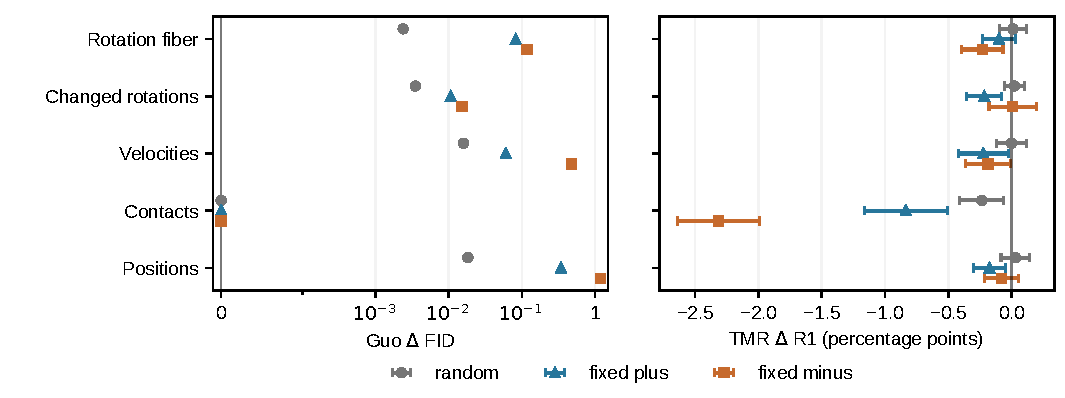
\includegraphics[width=\textwidth]{figures/matched_blocks.pdf}
\caption{\textbf{Equal-budget controls for every feature block.} Per-clip normalized $L_2$ change $\kappa\sqrt L$ with $\kappa=3$, using each evaluator's own normalization; random and both fixed signs over twenty draws. Only the fiber interventions preserve rotations and every other block; other block-only controls can be physically inconsistent with the unchanged blocks. The T2M evaluator excludes contacts. The axis label ``Guo'' denotes the T2M evaluator.}\label{fig:allblocks}\end{figure*}
\begin{table*}[t]
\centering\small
\caption{\textbf{T2M fixed directions, all twenty draws.} Both signs and radii; paired $t_{19}$ intervals adjust 32 endpoints in this primary family. Directions are fixed in time, but held-fixed feature blocks may be physically inconsistent. T2M excludes contacts; TMR reads all 263 channels.}\label{tab:table_coherent_guo_fixed}
\begin{tabular}{@{}llrrrr@{}}\toprule
$\kappa$&Intervention&$\Delta$ FID&95\% interval&$\Delta$ R1 (pp)&95\% interval\\\midrule
1&Rotations $+$&+0.00086&$[+0.00086,+0.00087]$&-0.038&$[-0.186,+0.110]$\\
1&Rotations $-$&+0.00102&$[+0.00102,+0.00103]$&+0.064&$[-0.106,+0.233]$\\
1&Velocities $+$&+0.00790&$[+0.00787,+0.00793]$&-0.073&$[-0.280,+0.133]$\\
1&Velocities $-$&+0.01773&$[+0.01767,+0.01779]$&-0.071&$[-0.257,+0.115]$\\
1&Contacts $+$&+0.00000&$[-0.00000,+0.00000]$&+0.000&$[+0.000,+0.000]$\\
1&Contacts $-$&+0.00000&$[-0.00000,+0.00000]$&+0.000&$[+0.000,+0.000]$\\
1&Positions $+$&+0.02842&$[+0.02832,+0.02852]$&+0.147&$[-0.061,+0.354]$\\
1&Positions $-$&+0.04435&$[+0.04424,+0.04447]$&-0.312&$[-0.566,-0.059]$\\
3&Rotations $+$&+0.01061&$[+0.01056,+0.01066]$&-0.184&$[-0.467,+0.099]$\\
3&Rotations $-$&+0.01512&$[+0.01507,+0.01517]$&+0.165&$[-0.057,+0.386]$\\
3&Velocities $+$&+0.06033&$[+0.06020,+0.06046]$&-0.247&$[-0.577,+0.083]$\\
3&Velocities $-$&+0.47604&$[+0.47496,+0.47712]$&-0.945&$[-1.293,-0.597]$\\
3&Contacts $+$&+0.00000&$[-0.00000,+0.00000]$&+0.000&$[+0.000,+0.000]$\\
3&Contacts $-$&+0.00000&$[-0.00000,+0.00000]$&+0.000&$[+0.000,+0.000]$\\
3&Positions $+$&+0.34160&$[+0.34071,+0.34249]$&-0.700&$[-1.107,-0.294]$\\
3&Positions $-$&+1.18896&$[+1.18691,+1.19101]$&-2.524&$[-2.917,-2.131]$\\
\bottomrule\end{tabular}\end{table*}

\begin{table*}[t]
\centering\small
\caption{\textbf{TMR fixed directions, all twenty draws.} Both signs and radii; paired $t_{19}$ intervals adjust 32 endpoints in this primary family. Directions are fixed in time, but held-fixed feature blocks may be physically inconsistent. Guo excludes contacts; TMR reads all 263 channels.}\label{tab:table_coherent_tmr_fixed}
\begin{tabular}{@{}llrrrr@{}}\toprule
$\kappa$&Intervention&$\Delta$ cosine&95\% interval&$\Delta$ R1 (pp)&95\% interval\\\midrule
1&Rotations $+$&-0.00048&$[-0.00052,-0.00045]$&-0.015&$[-0.094,+0.064]$\\
1&Rotations $-$&-0.00005&$[-0.00008,-0.00001]$&+0.015&$[-0.073,+0.103]$\\
1&Velocities $+$&-0.00074&$[-0.00078,-0.00070]$&+0.005&$[-0.083,+0.094]$\\
1&Velocities $-$&-0.00020&$[-0.00024,-0.00016]$&-0.036&$[-0.130,+0.059]$\\
1&Contacts $+$&-0.00034&$[-0.00047,-0.00021]$&+0.061&$[-0.140,+0.263]$\\
1&Contacts $-$&-0.00605&$[-0.00620,-0.00590]$&-0.353&$[-0.529,-0.178]$\\
1&Positions $+$&-0.00019&$[-0.00024,-0.00014]$&-0.036&$[-0.137,+0.066]$\\
1&Positions $-$&-0.00081&$[-0.00085,-0.00076]$&-0.012&$[-0.105,+0.081]$\\
3&Rotations $+$&-0.00319&$[-0.00331,-0.00308]$&-0.217&$[-0.355,-0.079]$\\
3&Rotations $-$&-0.00173&$[-0.00183,-0.00163]$&+0.009&$[-0.179,+0.196]$\\
3&Velocities $+$&-0.00522&$[-0.00535,-0.00508]$&-0.224&$[-0.421,-0.028]$\\
3&Velocities $-$&-0.00378&$[-0.00392,-0.00364]$&-0.186&$[-0.366,-0.007]$\\
3&Contacts $+$&-0.01998&$[-0.02030,-0.01966]$&-0.835&$[-1.163,-0.507]$\\
3&Contacts $-$&-0.04677&$[-0.04726,-0.04629]$&-2.316&$[-2.640,-1.991]$\\
3&Positions $+$&-0.00375&$[-0.00392,-0.00359]$&-0.175&$[-0.300,-0.049]$\\
3&Positions $-$&-0.00552&$[-0.00564,-0.00540]$&-0.081&$[-0.215,+0.053]$\\
\bottomrule\end{tabular}\end{table*}

\begin{table*}[t]
\centering\small
\caption{\textbf{T2M fixed minus random, all twenty draws.} Both signs and radii; paired $t_{19}$ intervals adjust 32 endpoints in this secondary contrast family. Directions are fixed in time, but held-fixed feature blocks may be physically inconsistent. T2M excludes contacts; TMR reads all 263 channels.}\label{tab:table_coherent_guo_contrast}
\begin{tabular}{@{}llrrrr@{}}\toprule
$\kappa$&Intervention&$\Delta$ FID&95\% interval&$\Delta$ R1 (pp)&95\% interval\\\midrule
1&Rotations $+$&+0.00080&$[+0.00080,+0.00081]$&-0.059&$[-0.216,+0.098]$\\
1&Rotations $-$&+0.00096&$[+0.00096,+0.00097]$&+0.042&$[-0.123,+0.207]$\\
1&Velocities $+$&+0.00772&$[+0.00770,+0.00775]$&-0.096&$[-0.263,+0.071]$\\
1&Velocities $-$&+0.01755&$[+0.01749,+0.01761]$&-0.094&$[-0.303,+0.116]$\\
1&Contacts $+$&+0.00000&$[-0.00000,+0.00000]$&+0.000&$[+0.000,+0.000]$\\
1&Contacts $-$&+0.00000&$[-0.00000,+0.00000]$&+0.000&$[+0.000,+0.000]$\\
1&Positions $+$&+0.02821&$[+0.02810,+0.02831]$&+0.098&$[-0.136,+0.332]$\\
1&Positions $-$&+0.04414&$[+0.04402,+0.04425]$&-0.361&$[-0.586,-0.136]$\\
3&Rotations $+$&+0.00712&$[+0.00704,+0.00719]$&-0.221&$[-0.499,+0.057]$\\
3&Rotations $-$&+0.01162&$[+0.01154,+0.01170]$&+0.128&$[-0.081,+0.337]$\\
3&Velocities $+$&+0.04447&$[+0.04423,+0.04471]$&-0.224&$[-0.484,+0.036]$\\
3&Velocities $-$&+0.46018&$[+0.45917,+0.46120]$&-0.922&$[-1.239,-0.606]$\\
3&Contacts $+$&+0.00000&$[-0.00000,+0.00000]$&+0.000&$[+0.000,+0.000]$\\
3&Contacts $-$&+0.00000&$[-0.00000,+0.00000]$&+0.000&$[+0.000,+0.000]$\\
3&Positions $+$&+0.32334&$[+0.32225,+0.32443]$&-0.671&$[-1.008,-0.335]$\\
3&Positions $-$&+1.17070&$[+1.16865,+1.17274]$&-2.495&$[-2.863,-2.126]$\\
\bottomrule\end{tabular}\end{table*}

\begin{table*}[t]
\centering\small
\caption{\textbf{TMR fixed minus random, all twenty draws.} Both signs and radii; paired $t_{19}$ intervals adjust 32 endpoints in this secondary contrast family. Directions are fixed in time, but held-fixed feature blocks may be physically inconsistent. Guo excludes contacts; TMR reads all 263 channels.}\label{tab:table_coherent_tmr_contrast}
\begin{tabular}{@{}llrrrr@{}}\toprule
$\kappa$&Intervention&$\Delta$ cosine&95\% interval&$\Delta$ R1 (pp)&95\% interval\\\midrule
1&Rotations $+$&-0.00059&$[-0.00063,-0.00054]$&-0.027&$[-0.108,+0.054]$\\
1&Rotations $-$&-0.00015&$[-0.00018,-0.00011]$&+0.003&$[-0.094,+0.101]$\\
1&Velocities $+$&-0.00076&$[-0.00080,-0.00072]$&+0.006&$[-0.118,+0.131]$\\
1&Velocities $-$&-0.00022&$[-0.00027,-0.00017]$&-0.034&$[-0.131,+0.062]$\\
1&Contacts $+$&-0.00042&$[-0.00056,-0.00027]$&+0.060&$[-0.133,+0.253]$\\
1&Contacts $-$&-0.00612&$[-0.00627,-0.00598]$&-0.355&$[-0.544,-0.165]$\\
1&Positions $+$&-0.00028&$[-0.00034,-0.00023]$&-0.054&$[-0.166,+0.058]$\\
1&Positions $-$&-0.00090&$[-0.00096,-0.00085]$&-0.030&$[-0.145,+0.084]$\\
3&Rotations $+$&-0.00404&$[-0.00418,-0.00391]$&-0.239&$[-0.373,-0.105]$\\
3&Rotations $-$&-0.00258&$[-0.00268,-0.00248]$&-0.014&$[-0.206,+0.178]$\\
3&Velocities $+$&-0.00525&$[-0.00538,-0.00512]$&-0.223&$[-0.412,-0.034]$\\
3&Velocities $-$&-0.00382&$[-0.00398,-0.00365]$&-0.185&$[-0.344,-0.027]$\\
3&Contacts $+$&-0.01876&$[-0.01912,-0.01840]$&-0.600&$[-0.844,-0.356]$\\
3&Contacts $-$&-0.04555&$[-0.04598,-0.04513]$&-2.081&$[-2.344,-1.818]$\\
3&Positions $+$&-0.00445&$[-0.00464,-0.00426]$&-0.205&$[-0.361,-0.048]$\\
3&Positions $-$&-0.00622&$[-0.00640,-0.00605]$&-0.111&$[-0.274,+0.052]$\\
\bottomrule\end{tabular}\end{table*}


Each reader's primary family contains 32 endpoints: four blocks, two signs, two radii and two scores. Separate secondary 32-endpoint families compare each fixed intervention with its original random block control on the same cohorts. Paired $t_{19}$ intervals use Bonferroni adjustment within each family. The historical null/random family remains 28 endpoints; the two phases are not presented as one prospective test. Matched-reference real-data FID starts at zero by construction. Numerically negligible nonzero contact FID can arise in the distance computation despite bitwise-identical T2M embeddings.

All metric cells, primary intervals and fixed-minus-random contrasts are recomputed independently. Every saved per-clip norm is checked, and the first eight fixtures per condition/draw are reconstructed using separate formulas and SciPy rotations. Native forward checks verify the saved embeddings, including the T2M evaluator's caption/length reordering. Protected channels and padding are compared bitwise; the non-null rotation controls must change represented matrices. These checks do not claim complete geometry replay of unsaved arrays.

\begin{figure*}[t]\centering
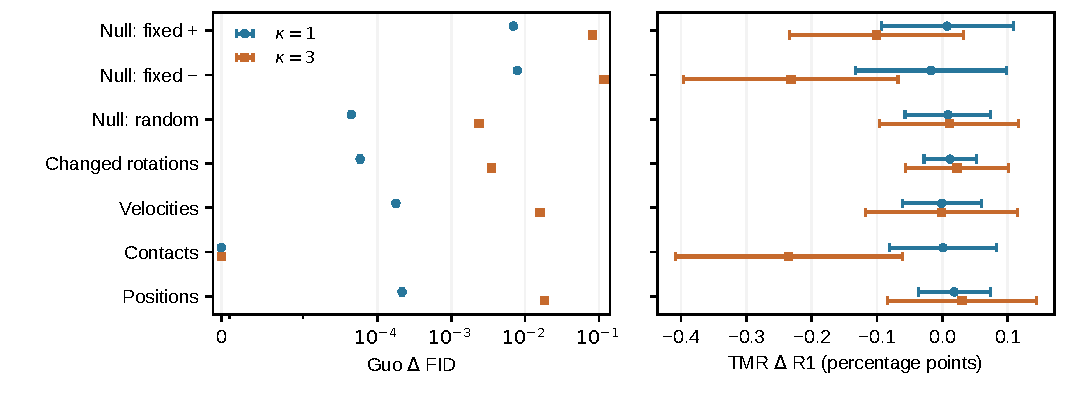
\includegraphics[width=\textwidth]{figures/matched_blocks_random.pdf}
\caption{\textbf{The original random/null controls, both radii.} All twenty draws; the historical 28-endpoint intervals remain unchanged. Here $\kappa$ denotes the numerical budget and $\rho$ remains the positive scale in the rotation fiber. Random position/velocity noise has a larger T2M FID effect than random fiber coefficients at the larger budget. The axis label ``Guo'' denotes the T2M evaluator. }\label{fig:randomblocks}
\end{figure*}


\section{Directional comparison within the rotation block}
For $\kappa=3$, fixed positive/negative fiber directions have mean T2M FID changes 0.082295/0.116879, versus 0.010609/0.015118 for fixed physical-rotation directions. With the same sign, the ratios of these mean changes are 7.757 and 7.731. Both experiments use the same 126-dimensional rotation block, normalizer, real cohorts and matched per-clip L2. This is a descriptive arithmetic comparison of frozen results, not a new prospective hypothesis test or a universal ranking of rotation directions. In particular, random fiber coefficients produce less FID change than the original random physical-rotation control.



\section{Native HumanML3D released-output audit}
\paragraph{Native loader, repeats and sample counts.}
This audit uses the public Text2MotionDatasetV2, including subcaption segments, random caption choice, and native single/double crops to multiples of four. There are 4,648 cached test entries and 4,640 after dropping the incomplete 32-item batch. Entry counts include segments and mirrored motions, rather than 4,640 independent recordings. Twenty seeds 1234--1253 control caption/crop draws; independent full real-reference draws use seed plus 100,000. Generation uses seed plus 200,000. MDM's native nominal 1,000 limit emits 1,024 outputs; other methods emit 4,640. Metrics use the same 32-candidate batches in raw/canonical comparisons. Unchanged outputs, captions and reference embeddings are shared between each pair.

\paragraph{Five public methods and inference parity.}
MDM50~\cite{tevet2023} uses 50 native steps, CFG 2.5 and CLIP-B/32. MLD~\cite{mld2023} uses DDIM 50, CFG 7.5 and CLIP-L/14; MotionLCM-v1~\cite{motionlcm2024} uses one LCM step, CFG 7.5 and Sentence-T5-large. T2M-GPT~\cite{t2mgpt2023} uses native categorical/EOS sampling, 512 VQ entries, block length 51 and the released net\_last decoder. Original T2M~\cite{guo2022} uses its recurrent prior and native duration estimator. Native component classes and strict states are retained. Throughput batching grows from 32 to 128 for MLD and GPT; the random draw order can differ, while evaluation batches remain 32. T2M batches share both motion and caption length because its attention does not mask padded caption positions. All valid repetitions remain included; no settings were chosen by test scores.

Synthetic native/batched checks give exact decoder/reverse agreement for MLD/LCM, at most $6.5\times 10^{-5}$ normalized mean-prior difference for the correct T2M grouping, and $5.7\times 10^{-4}$ for GPT convolution decoding. Batched floating-point arithmetic is not claimed bit-identical. Pinned author code, weight hashes, executed source versions and parity fixtures are included with the artifacts.

\paragraph{Metric uncertainty and reader replication.}
The primary reader is the official MDM-linked T2M evaluator. The official T2M-GPT download contains distinct encoder weights of the same architecture; native normalization arrays are equal. The secondary reader reuses every saved output and independent reference draw. Native mean intervals use $1.96\,\mathrm{std}_{0}/\sqrt{20}$. Paired gap intervals use $t_{19}$ with ten FID/R1 comparisons per reader; MM-distance is a separate five-comparison family. The two readers' families are reported separately. The repetitions describe generation and native draw variability on this public split, not independent corpora or pretraining uncertainty. No exact published-score reproduction is claimed.

\begin{table*}[t]
\centering\footnotesize
\caption{\textbf{Two official checkpoints, one evaluator architecture.} All five releases and 20 repetitions are retained. R1 uses native 32-candidate batches. Each reader uses a ten-endpoint FID/R1 interval family; these families are reported separately. GPT weights differ from the MDM-linked weights; the samples and normalization are shared. Intervals describe raw$-C$.}
\label{tab:releasereaders}
\begin{tabular}{llrrrrrr}\toprule
Reader&Release&Raw FID&$C$ FID&FID gap interval&Raw R1&$C$ R1&R1 gap interval\\\midrule
MDM&MDM50&0.4550&0.4504&$[+0.0035,+0.0058]$&0.4115&0.4115&$[-0.0017,+0.0018]$\\
MDM&MLD&0.4453&0.4491&$[-0.0052,-0.0024]$&0.4118&0.4105&$[+0.0003,+0.0023]$\\
MDM&MotionLCM-v1&0.5747&0.6062&$[-0.0347,-0.0282]$&0.4374&0.4350&$[+0.0005,+0.0043]$\\
MDM&T2M-GPT&0.1828&0.1488&$[+0.0325,+0.0354]$&0.4226&0.4240&$[-0.0030,+0.0002]$\\
MDM&T2M&1.3935&1.3471&$[+0.0441,+0.0486]$&0.3933&0.3930&$[-0.0009,+0.0017]$\\
GPT&MDM50&0.5129&0.5104&$[+0.0012,+0.0040]$&0.4586&0.4584&$[-0.0015,+0.0019]$\\
GPT&MLD&0.4206&0.4216&$[-0.0023,+0.0002]$&0.4669&0.4666&$[-0.0012,+0.0017]$\\
GPT&MotionLCM-v1&0.4195&0.4294&$[-0.0138,-0.0060]$&0.5042&0.5026&$[-0.0004,+0.0035]$\\
GPT&T2M-GPT&0.1204&0.1115&$[+0.0076,+0.0103]$&0.4909&0.4898&$[-0.0004,+0.0026]$\\
GPT&T2M&1.0836&1.0917&$[-0.0111,-0.0051]$&0.4547&0.4540&$[-0.0007,+0.0021]$\\
\bottomrule\end{tabular}\end{table*}

All five primary FID gap intervals exclude zero. Primary raw/canonical mean ordering is T2M-GPT, MLD, MDM, MotionLCM, T2M. Four secondary FID intervals exclude zero; MLD is inconclusive and T2M's gap changes direction. Secondary mean MLD/MotionLCM order differs across encodings by a small amount, but reliable ranking reversal was not established. All secondary R1 gap intervals include zero. This is score sensitivity across official weights, not a claim that canonicalization always improves metrics.

\paragraph{Full native fixed controls and physical verification.}
Across 20 full reference repetitions, mean real-motion FID is 0.000990 before recoding and 0.000990 after canonicalization. Fixed directional $+0.1/-0.1$ gives 0.06129/0.08336, $+0.35/-0.35$ gives 2.00261/3.63852, and random 0.35 gives 0.02628. The real draws are independent in crop/caption order, explaining the nonzero baseline; these numbers are distinct from the paired-subset FID-zero controls below. Strong directional shifts do not imply natural prevalence at that magnitude.

Independent native conversion checks all 391,680 release raw/canonical pairs; maximum double-precision angle is $3.6\times 10^{-6}$ degrees, while the largest native float32 matrix residual is $2.0\times 10^{-5}$ for near-degenerate features. Every nonrotation channel is bitwise unchanged. Two native FK pairs per release/repetition give 200 sampled pairs and maximum position error $9.6\times 10^{-7}$. The complete saved-embedding FID/R1 endpoints are recomputed independently. Real fixed-control geometry receives additional native checks; it is not inferred from embedding equality.


\section{Additional public releases and native KIT-ML}
\begin{table*}[t]
\centering\footnotesize
\caption{\textbf{Additional releases and KIT.} All 20 draws, own native evaluator normalization, same-output raw/C. Intervals for raw$-C$ adjust ten FID/R1 comparisons. HumanML MoMask uses 4,640 outputs; MotionDiffuse/DiP use 1,024 with full reference. KIT uses 704 outputs/reference. DiP is prefix-conditioned; published-score reproduction is not claimed.}\label{tab:additionalfull}
\begin{tabular}{@{}lrrrrrr@{}}\toprule
Data/release&Raw FID&$C$ FID&FID gap interval&Raw R1&$C$ R1&R1 gap interval\\\midrule
humanml/MoMask&0.0677&0.0644&$[+0.00279,+0.00382]$&0.4632&0.4626&$[-0.0010,+0.0023]$\\
humanml/DiP (prefix)&0.3665&0.3650&$[+0.00004,+0.00303]$&0.4518&0.4518&$[-0.0022,+0.0023]$\\
humanml/MotionDiffuse&0.9766&0.9807&$[-0.00737,-0.00076]$&0.4277&0.4273&$[-0.0018,+0.0026]$\\
kit/MoMask&0.3512&0.3649&$[-0.02473,-0.00270]$&0.4175&0.4181&$[-0.0070,+0.0057]$\\
kit/MotionDiffuse&1.7794&1.8159&$[-0.04282,-0.03002]$&0.4125&0.4116&$[-0.0017,+0.0036]$\\
\bottomrule\end{tabular}\end{table*}

MoMask~\cite{momask2024} uses the released residual VQ model, latest masked-transformer checkpoint and best-FID residual checkpoint. Inference uses 18 mask steps, CFG 4, temperature 1, top-k threshold 0.9, no Gumbel sampling, then residual CFG 5. The native decoder and its normalization remain unchanged. Prescribed durations are supplied; future source poses are not inputs. Both HumanML3D and native KIT use the full eligible test cohorts after dropping the incomplete 32-item batch, with 20 draws.

MotionDiffuse~\cite{motiondiffuse2024} uses the author encoder and normalization, native linear 1000-step DDPM, epsilon prediction and fixed-small variance. Prescribed durations follow the native 40-frame HumanML/24-frame KIT minimum. An elementwise-equivalent device mask removes the upstream Python frame loop; mask/full-forward equality is checked. Compilation retains all native layers, weights and float32 operations with TF32 disabled. Operator fusion changes rounding slightly, so compiled/eager parity residuals are reported, rather than claiming bit identity. Inference batches are 128; HumanML outputs are capped at 1,024 with a full reference, and KIT uses the full 704-output cohort. These are paired consistency audits, not an exact reproduction of published scores.

DiP~\cite{closd2025} uses the no-target author checkpoint at 200,000 steps with EMA, DistilBERT and native autoregressive sampling: context 20, prediction 40, 10 diffusion steps, CFG 7.5. The first 20 frames of each saved cropped source motion initialize its prefix, excluded from the generated output. No future source frames are passed. This prefix-conditioned setting differs from text-only generation and is not a claim that DiP constitutes an unrelated MDM architecture. Twenty 1,024-output draws use full real references.

Native KIT~\cite{kit2016} uses the official processed MMM archive and its 251-feature T2M evaluator. Its 20 local 6D rotations occupy 64:184; the evaluator excludes the final four contact channels. Its real test reference and outputs contain 704 native entries per draw, including segment annotations. The separate TMR KIT AMASS model consumes 263 features and is incompatible with this archive. It is not substituted or padded to accept 251 features.

All raw/canonical pairs share emitted arrays, captions, masks, candidate groups and reference. Additional-release uncertainty is analyzed jointly within its comparison family; absolute signed differences remain separate from published mean margins. Sources, archive hashes, native-component checks and complete output arrays accompany the artifacts. Native KIT coordinates differ in scale from HumanML meters, so its FK residuals are reported in native units and relative to body height; KIT inputs are never rescaled before evaluation.


\section{Published-score scale context}
\begin{table*}[t]
\centering\footnotesize
\caption{\textbf{Published margins give scale, not paired significance.} Author-reported FID and its reported 95\% mean margin, beside our signed same-output raw$-C$ gap. Original five rows use HumanML3D; other datasets are labeled. Samples, readers, checkpoints and conditioning differ. MDM50/DiP use corrected author results; T2M uses estimated length. DiP is prefix-conditioned. These numbers do not test our gap against a published uncertainty or establish leaderboard reproduction.}\label{tab:publishedscale}
\begin{tabular}{@{}lrr@{}}\toprule
Method/dataset/setting&Published FID&Our raw$-C$\\\midrule
MDM50, corrected release~\cite{tevet2023}&$0.489\pm0.047$&+0.0046\\
MLD~\cite{mld2023}&$0.473\pm0.013$&-0.0038\\
MotionLCM, one step~\cite{motionlcm2024}&$0.467\pm0.012$&-0.0315\\
T2M-GPT, $\tau\sim U[0,1]$~\cite{t2mgpt2023}&$0.141\pm0.005$&+0.0340\\
T2M, estimated length~\cite{guo2022}&$1.087\pm0.021$&+0.0464\\
MoMask / HumanML~\cite{momask2024}&$0.045\pm0.002$&+0.0033\\
DiP / HumanML, corrected release~\cite{closd2025}&$0.228\pm0.027$&+0.0015\\
MotionDiffuse / HumanML, preprint~\cite{motiondiffuse2024}&$0.630\pm0.001$&-0.0041\\
MoMask / KIT, final table~\cite{momask2024}&$0.204\pm0.011$&-0.0137\\
MotionDiffuse / KIT, preprint~\cite{motiondiffuse2024}&$1.954\pm0.062$&-0.0364\\
\bottomrule\end{tabular}\end{table*}

Published FID margins contextualize the absolute representation changes (\cref{tab:publishedscale}). They estimate uncertainty of different means under different protocols; they are not uncertainties of our paired gaps. No cross-paper significance test follows. The T2M-GPT uniform-corruption, MLD and one-step MotionLCM rows come from their respective papers. T2M uses its estimated-length result, $1.087\pm0.021$; the separate real-length row is $1.067\pm0.002$.

MoMask uses the final CVPR table, including KIT $0.204\pm0.011$ rather than the abstract's 0.228. MotionDiffuse scale values come from the 2022 author preprint associated with its public release (\url{https://arxiv.org/abs/2208.15001}); the bibliography cites its journal publication. DiP's corrected author table reports $0.228\pm0.027$. Our checkpoint and prefix setting are recorded separately. These numerical sources provide scale context, not proof that our inference settings reproduce each published experiment.

MDM50's corrected $0.489\pm0.047$ comes from the authors' maintained results rather than the original 1000-step paper row. The pinned release includes the result at \url{https://github.com/GuyTevet/motion-diffusion-model/blob/ef8edce6a53c6ab19e53b4d4dcf15bc0bc60a778/assets/fixed_results.tex}; its revision and fingerprint are recorded with the artifacts. We do not mix the old paper margin with this 50-step checkpoint or interpret the published score as a reproduction target for our capped-output audit.


\section{Natural rotation deviations and model-family mechanism}
\begin{figure}[t]\centering
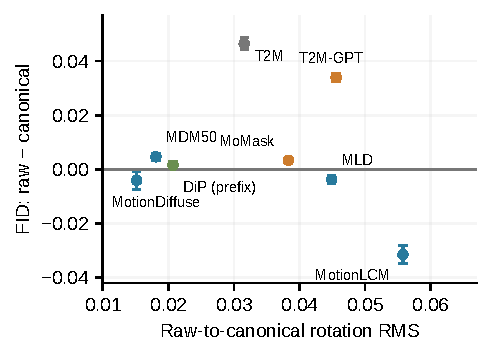
\includegraphics[width=\columnwidth]{figures/rotation_mechanism.pdf}
\caption{\textbf{Natural rotation deviations do not impose a uniform penalty.} Signed raw-minus-canonical T2M FID gaps against valid-frame raw-to-canonical rotation RMS for all eight HumanML3D release settings, with paired family-adjusted intervals. Blue: diffusion/consistency; orange: VQ; gray: VAE; green: prefix-conditioned. Family and conditioning are confounded; this is descriptive.}\label{fig:mechanism}\end{figure}

All eight HumanML3D releases appear in the mechanism analysis. Four unconditioned diffusion/consistency releases are compared descriptively with two VQ releases; T2M's VAE and prefix-conditioned DiP are shown separately. RMS is the square root of mean squared raw-to-canonical change over all valid 126 rotation values, first aggregated within each draw and then across twenty draws. It is not full-feature RMS or a norm including padding. Newly added releases use all saved outputs; earlier verified geometric records supply the original five.

Signed family means are $-0.00867$ FID for the four diffusion/consistency settings and $+0.01864$ for the two VQ settings. These are not estimates from independent model-family training replicas. T2M has the largest positive gap overall, $+0.04636$; prefix-conditioned DiP is separate. Three diffusion/consistency gaps are negative and one positive. Thus removing within-rotation noncanonicality does not uniformly favor diffusion in these releases.

Across eight release means, Spearman correlation of RMS with signed gap is $-0.095$ and with absolute gap $0.286$. Exact two-sided permutation $p$ values are 0.840 and 0.501; both adjusted values are 1.0. This small, confounded release-level analysis supplies no evidence of a monotone relation and cannot establish independence. It concerns only the exact rotation fiber and neither tests velocity/contact errors nor refutes MARDM's full representation/distribution and diffusion-training mechanism. All per-draw RMS values and original score intervals are preserved with the artifacts.


\section{Public essential-feature evaluator comparison}
\begin{table*}[t]
\centering\small
\caption{\textbf{Common-reference essential-reader comparison.} Mean embedding FID with nominal $t_{19}$ 95\% intervals over all twenty draws. The same saved real cohort is encoded separately by each reader; T2M is re-scored with this reference, which differs from its original independent-reference audit. FID scales differ across reader weights and architectures. E-CLIP FID is descriptive, not an official generation metric.}\label{tab:mardmfull}
\begin{tabular}{@{}lrrrr@{}}\toprule
Release&T2M raw&T2M $\C$&E-GRU&E-CLIP\\\midrule
MoMask&$0.0678\, [0.0651,0.0704]$&$0.0644\, [0.0618,0.0670]$&$0.0459\, [0.0432,0.0487]$&$0.0052\, [0.0050,0.0053]$\\
T2M-GPT&$0.1829\, [0.1765,0.1893]$&$0.1489\, [0.1431,0.1547]$&$0.4013\, [0.3201,0.4826]$&$0.0079\, [0.0077,0.0080]$\\
DiP (prefix)&$0.3665\, [0.3175,0.4155]$&$0.3650\, [0.3166,0.4133]$&$0.3299\, [0.2905,0.3693]$&$0.0160\, [0.0151,0.0169]$\\
MLD&$0.4446\, [0.4336,0.4556]$&$0.4483\, [0.4372,0.4595]$&$0.4269\, [0.4129,0.4410]$&$0.0166\, [0.0163,0.0168]$\\
MDM50&$0.4540\, [0.4221,0.4859]$&$0.4494\, [0.4178,0.4810]$&$0.4555\, [0.4200,0.4911]$&$0.0246\, [0.0238,0.0255]$\\
MotionLCM&$0.5740\, [0.5614,0.5867]$&$0.6055\, [0.5916,0.6194]$&$0.6125\, [0.5922,0.6329]$&$0.0188\, [0.0184,0.0191]$\\
MotionDiffuse&$0.9752\, [0.8845,1.0659]$&$0.9793\, [0.8897,1.0689]$&$1.0269\, [0.9385,1.1153]$&$0.0383\, [0.0367,0.0399]$\\
T2M&$1.3914\, [1.3648,1.4180]$&$1.3450\, [1.3181,1.3719]$&$0.9966\, [0.9720,1.0212]$&$0.0319\, [0.0316,0.0323]$\\
\bottomrule\end{tabular}\end{table*}

\begin{table}[t]
\centering\footnotesize
\caption{\textbf{Essential-only evaluation is a different remedy.} Within-reader ranks of mean embedding FID over twenty common-reference draws. Guo $\C$ retains rotations; MARDM GRU/CLIP use 67 essential features. CLIP FID is descriptive. Ranks compare these saved release settings, not published leaderboards or evaluator accuracy.}\label{tab:mardmranks}
\begin{tabular}{@{}lrrr@{}}\toprule
Release&Guo $\C$&E-GRU&E-CLIP\\\midrule
MoMask&1&1&1\\
T2M-GPT&2&3&2\\
DiP (prefix)&3&2&3\\
MLD&4&4&4\\
MDM50&5&5&6\\
MotionLCM&6&6&5\\
MotionDiffuse&7&8&8\\
T2M&8&7&7\\
\bottomrule\end{tabular}\end{table}

The public MARDM~\cite{mardm2025} checkpoint contains a 67-feature GRU reader and a motion/text Transformer contrastive reader. Both use the author normalization for root/local position features. Native layers and public states are loaded strictly. The CLIP constructor's unused visual tower is avoided using only token/position embedding placeholders; the released state then overwrites every parameter, checked bitwise before inference. No forward operation or fitted weight is replaced.

All eight saved releases and twenty original draws are evaluated without generation or training. A common saved real cohort is separately encoded by every reader. T2M scores are recomputed against the same real cohort rather than its original independent real-reference draw, so the values in \cref{tab:mardmfull} differ slightly from the original release audit. MDM, MotionDiffuse and DiP have 1,024 outputs; other releases have 4,640. DiP remains prefix-conditioned. Within each reader, rankings use twenty-draw mean embedding FID. Essential-CLIP FID is descriptive latent distance, not an official leaderboard metric, and its numerical scale cannot be compared with GRU/T2M FID.

Changing only rotation coordinates leaves the first 67 input values bitwise fixed. Native repeated forwards on the first 32 outputs of every release/draw give exactly equal essential-reader embeddings. This expected structural invariance is not an accuracy-cost test. Canonical T2M retains rotations and has the same mean ordering as raw T2M here; essential GRU changes the DiP/T2M-GPT and T2M/MotionDiffuse ordering, while essential CLIP changes MDM/MotionLCM and T2M/MotionDiffuse. Both have Kendall agreement 0.857 with canonical T2M. The ranking differences combine feature selection, architecture and different fitted weights; they cannot be attributed solely to removal of rotation redundancy or interpreted as a reliable leaderboard reversal.

All 640 saved metric cells, mean intervals and rankings are recomputed independently. Native parameter/state checks and first/last-draw inference fixtures verify the released computation. For the rotation-only sign-language representations, an essential-only input analogous to discarding HumanML3D rotations would remove all movement features. Canonicalization instead retains every represented joint rotation; its accuracy remains a separate empirical question.


\section{TMR: an independent Transformer evaluator}
\begin{table*}[t]
\centering\footnotesize
\caption{\textbf{Different architecture, modest natural dependence.} Native TMR cosine/sample-mean inference on compatible existing cohorts; 20 draws, family12 intervals for raw$-C$. This is not the full official annotation/filter protocol.}\label{tab:tmrnatural}
\begin{tabular}{@{}lrrrrrr@{}}\toprule
Source&Raw R1&$C$ R1&R1 gap interval&Raw cosine&$C$ cosine&Cosine gap interval\\\midrule
Real&0.6784&0.6784&$[+0.0000,+0.0000]$&0.5245&0.5245&$[-0.00000,+0.00000]$\\
MDM50&0.5578&0.5571&$[-0.0015,+0.0029]$&0.4296&0.4299&$[-0.00040,-0.00016]$\\
MLD&0.5848&0.5841&$[-0.0005,+0.0019]$&0.4527&0.4526&$[+0.00002,+0.00024]$\\
MotionLCM-v1&0.6785&0.6757&$[+0.0013,+0.0043]$&0.5035&0.5024&$[+0.00098,+0.00132]$\\
T2M-GPT&0.6703&0.6698&$[-0.0006,+0.0017]$&0.5335&0.5331&$[+0.00035,+0.00057]$\\
T2M&0.5626&0.5611&$[+0.0003,+0.0028]$&0.4331&0.4311&$[+0.00182,+0.00208]$\\
\bottomrule\end{tabular}\end{table*}

TMR~\cite{tmr2023} uses author ACTOR motion/text encoders with six Transformer layers and 256 latent dimensions. Motion input has 263 features and the author mean/std with epsilon $10^{-12}$. Frozen DistilBERT supplies 768-dimensional token embeddings. Native deterministic inference takes the VAE mean token; similarity is normalized cosine. Author weights are loaded strictly and the archive's supplied MD5 is verified.

The natural audit reuses the original five public generators and real-motion cohorts across 20 draws. Raw/canonical, fixed $\pm 0.1/\pm 0.35$ and random 0.35 are all scored. Random fields use seed 42 plus global clip index, independently per record, differing from the T2M fixed-control field. Twelve paired R1/cosine endpoints use family-adjusted$t_{19}$ intervals. We retain the compatible T2M-feature cohorts, candidate batches of 32 and their annotations rather than reproduce TMR's full AMASS annotation/semantic-filter protocol. In particular, no semantic-neighbor filter or full-gallery retrieval score is claimed.

Natural R1 differences are small: MotionLCM and T2M have positive intervals; other generated-source intervals include zero. Matched cosine detects additional changes but is a separate endpoint. Real R1 is identical before/after canonicalization. Saved scores, native forward outputs and batch/serial motion embeddings are independently checked. DistilBERT padding/batch changes cause float32 text differences below $4.7\times 10^{-5}$; matching the producer's 64-caption cache batches reproduces saved vectors. This arithmetic diagnostic is not a new evaluation protocol.

\begin{table*}[t]
\centering\small
\caption{\textbf{All TMR attack controls on 1,024 clips/source.} Wrong targets are a circular caption shift. The generic attack matches the rotation-fiber attack\'s per-clip standardized L2 radius while changing continuous features. Canonical source and attacked R1 agree within each source; raw/canonical source scores may differ.}\label{tab:tmrattackfull}
\begin{tabular}{@{}llrrrr@{}}\toprule
Source&Condition&Actual R1&Wrong R1&$\C$ actual R1&Actual cosine\\\midrule
Real&original&0.688&---&0.688&0.524\\
Real&actual target&1.000&0.000&0.688&0.944\\
Real&wrong target&0.015&0.968&0.688&0.140\\
Real&canonical gradient&0.688&0.010&0.688&0.524\\
Real&generic L2&1.000&---&1.000&0.991\\
MDM&original&0.578&---&0.580&0.426\\
MDM&actual target&0.993&0.000&0.580&0.920\\
MDM&wrong target&0.022&0.946&0.580&0.146\\
MDM&canonical gradient&0.578&0.017&0.580&0.426\\
MDM&generic L2&1.000&---&1.000&0.991\\
\bottomrule\end{tabular}\end{table*}

Capability tests use all 1,024 fixed clips per source of the fixed caption-targeted cohort, with real and MDM sources, 80 Adam steps, learning rate 0.1, bound 0.35 and final iterate. The reader remains frozen. Targets are actual or circularly shifted captions; the canonical-gradient control differentiates through canonical input. Every target/canonical endpoint is included. The source clips now match the T2M cohort; native cosine similarity and candidate permutations still differ, preventing an across-architecture accuracy ranking.

Actual-target R1 changes 0.688 to 1.000 on real motion and 0.578 to 0.993 on MDM; wrong targets also redirect retrieval while actual-target agreement decreases. Canonical embeddings change by at most $6.7\times 10^{-6}$. Canonical MDM R1 is 0.580 both before and after recoding, distinct from source raw R1 0.578. Independent native checks cover 6,144 clip pairs and 48 FK samples: maximum angle $2.0\times 10^{-5}$ degrees, maximum FK displacement $9.6\times 10^{-7}$ m, bitwise protected channels and unchanged padding.

\paragraph{Generic adversary at matched L2.}
For each clip, we measure the actual-target rotation-fiber attack's L2 radius in TMR-normalized units over valid frames. A generic 80-step Adam attack changes all 259 continuous features, keeps contacts/padding fixed and projects onto that per-clip radius after every update. It reaches perfect retrieval and remains effective under canonicalization. Mean RIC position changes are 0.810 m real/0.899 m MDM, and mean rotation changes are 25.2/25.7 degrees. The features can be physically inconsistent across blocks. This comparison does not claim a smallest physical adversary; it demonstrates the distinct guarantee of zero physical change inside the rotation fiber. Verified radius excess is at most $3.1\times 10^{-5}$ normalized units.


\section{Physical angular sensitivity}
\begin{table}[t]
\centering\footnotesize
\caption{\textbf{Coherent physical calibration.} Means across 20 full real cohorts; paired coherent zero reference, common four-frame crop. Original-to-zero cost is explicit. Doses are local nonroot rotation angles, with fixed-per-clip or independent-per-frame axes. All recodings preserve that reconstructed movement.}\label{tab:physicalcal}
\begin{tabular}{@{}lrrr@{}}\toprule
Condition&FID&R1&MM-dist.\\\midrule
Original vs reconstruction&0.02006&0.4510&3.2545\\
Coherent zero&3.353e-10&0.4474&3.2707\\
$C$ of coherent zero&1.74e-10&0.4474&3.2707\\
Fixed recoding $+0.1$&0.05898&0.4461&3.2749\\
Fixed recoding $-0.1$&0.08278&0.4386&3.3222\\
Fixed recoding $+0.35$&1.972&0.3900&3.7303\\
Fixed recoding $-0.35$&3.574&0.3565&3.9646\\
Random recoding $0.35$&0.02445&0.4418&3.2952\\
Fixed axes, $0.1^\circ$&3.661e-07&0.4474&3.2707\\
Fixed axes, $0.3^\circ$&3.476e-06&0.4474&3.2707\\
Fixed axes, $1^\circ$&6.385e-05&0.4475&3.2707\\
Fixed axes, $3^\circ$&0.002647&0.4468&3.2723\\
Fixed axes, $10^\circ$&0.2996&0.4268&3.3625\\
Fixed axes, $30^\circ$&14.44&0.2432&5.4553\\
Framewise axes, $0.1^\circ$&1.624e-05&0.4474&3.2708\\
Framewise axes, $0.3^\circ$&0.001198&0.4485&3.2718\\
Framewise axes, $1^\circ$&0.3502&0.4408&3.3283\\
Framewise axes, $3^\circ$&10.24&0.3621&4.3791\\
Framewise axes, $10^\circ$&38.98&0.2186&6.5188\\
Framewise axes, $30^\circ$&75.17&0.0970&8.7587\\
\bottomrule\end{tabular}\end{table}

We perturb the 21 nonroot rotations using local SO(3) angles 0.1/0.3/1/3/10/30 degrees. Gaussian random axes are normalized per joint, either fixed throughout a clip or independently drawn at each frame. Axes share seeds across angle doses, with deterministic per-record indexing, and both noise modes use all 20 saved real test cohorts. No angle or clip is selected by a score.

Forward kinematics uses the native skeleton and each clip's initial bone lengths. Root trajectory stays fixed. Rotations, RIC positions, root-local joint velocities and native foot-contact predicates are updated together. A common four-frame crop supplies next-frame positions for velocities. The reference is the paired coherent zero-angle reconstruction; its FID-zero baseline is therefore by construction. Original-to-reconstruction FID is 0.0201 and R1 changes 0.4510$\to$0.4474, so reconstruction cost is not hidden.

On this same coherent reference, fixed $+0.35/-0.35$ recodings give FID 1.972/3.574 with zero physical change. These levels lie between the measured 1- and 3-degree frame-independent doses, but between 10 and 30 degrees with temporally fixed axes. These are brackets on the measured curves, not a universal degree equivalence, perceptual claim or result of new interpolated-dose experiments. Full FID/R1/MM curves, small/random recodings and nominal$t_{19}$ mean intervals are reported.

Independent checks verify 240 physical clip cases, native SO(3) angles, RIC/FK agreement, recomputed local velocities/contacts, fixed roots and padding. Saved metric endpoints are recomputed against their exact references. The reconstruction follows native geometry conventions; it is not a licensed SMPL mesh or human-quality calibration.


\section{HumanML3D caption-targeted controls}
\paragraph{Representation and native inference.}
HumanML3D~\cite{guo2022} has root features 0--3, relative positions 4--66, 21 continuous rotations 67--192, velocities 193--258 and foot contacts 259--262. Its native converter uses the first two matrix columns. The released movement encoder consumes features 0--258 without a rotation projection. We alter only 67--192 before normalization, then use the released evaluation mean/std and remask padded frames. Position-based reconstruction ignores the altered block; native FK additionally verifies rotation-based reconstruction. Other feature channels are checked bitwise, separately from floating-point matrix equality.

Public T2M weights come from the MDM evaluator download script; all three frozen encoder states load strictly into the author architecture. The native MDM evaluation wrapper and our ordering-preserving adapter agree within $4.8\times 10^{-7}$ on validation fixtures. Native R-precision, MM-distance and FID match saved metrics. The encoder reads 259 channels, not a canonicalized or position-only replacement. Source hash inventories identify the pinned author code and checkpoints.

\paragraph{Data origin and fixed subsets.}
We use a public mirror of the processed motion pinned by revision and SHA256; its 4,297,557,992-byte size matches the author-linked inventory. The mirror's 012314 example is float64 while the author Git example is float32: maximum/RMS differences are $1.94\times 10^{-5}$/$7.67\times 10^{-7}$. This is numerical compatibility, not proof of byte identity for the full archive. Author text/split files and normalization are used. All motion matrices and physical controls are checked on the actual saved inputs.

Eligible full-caption clips have 40--199 frames. Selection seed 20261012 samples 128 VAL and 1,024 test clips without replacement, with fixed caption draws and crops to multiples of four. These are subset audits, not full-score leaderboard reproductions. Real and generated inputs use the same captions and durations. MDM50~\cite{tevet2023} uses the official encoder checkpoint, 50 native sampling steps, CFG 2.5 and seed 42. No reference poses enter generation. An unused mesh constructor is disabled; denoiser, CLIP and diffusion operations and parameters are unchanged.

\paragraph{Attack and scoring.}
Nine fixed controls include identity, canonicalization, signed global bounds 0.05/0.1/0.35 and seeded random coefficients. Per-clip attacks optimize actual or shifted-caption embedding distance using 80 final Adam steps, learning rate 0.1, zero initialization and coefficient bound 0.35. A third control applies the loss after canonicalization. Evaluator weights remain frozen. A no-dropout recurrent flag enables input gradients; forward parity is checked and final scoring uses eval mode. Shifted text changes the optimization target without changing motion.

R-precision top 1 averages five fixed 32-candidate permutations (seeds 11/97/909/1337/2027). FID always compares motion embeddings with a fixed real-reference subset. The target-caption objective improves retrieval and MM-distance while worsening FID; no metric is interpreted as a human-quality gain at unchanged physical motion. All fixed controls and both splits are in \cref{tab:humanmlfixed}; test attack/control endpoints are in \cref{tab:humanmlfull}. Original/mirrored IDs are grouped for 10,000 paired bootstrap draws; six source/attack endpoints are adjusted together. These intervals condition on the five fixed candidate pools and one generator seed, not unseen evaluators or pretraining variability.

\begin{table}[t]\centering\small
\caption{\textbf{HumanML3D attack and canonical-loss controls.} Full fixed test subset, 1,024 clips per source. R1/MM use the row's target (source caption for Source/Actual; shifted caption for Shifted/Can. loss). FID always uses the fixed real-motion reference. The target-caption attack improves retrieval while worsening FID.}
\label{tab:humanmlfull}
\begin{tabular}{llrrr}\toprule
Source&Target/loss&R1&MM&FID\\\midrule
Real&Source&0.462&3.200&0.000\\
Real&Actual&0.996&0.613&1.311\\
Real&Shifted&0.839&1.479&2.247\\
Real&Can. loss&0.028&9.599&0.000\\
MDM50&Source&0.397&3.582&0.369\\
MDM50&Actual&0.993&0.659&1.287\\
MDM50&Shifted&0.788&1.821&2.352\\
MDM50&Can. loss&0.033&9.741&0.369\\
\bottomrule\end{tabular}\end{table}

\begin{table*}[t]\centering\small
\caption{\textbf{All target-independent HumanML3D encoding controls.} 128 VAL (DEV) and 1,024 TEST clips per source. Signed global coefficients are $(b,-b,b)$, with $b=\pm0.05,\pm0.1,\pm0.35$. No target text enters the transform. FID reference is the fixed real subset for each split.}
\label{tab:humanmlfixed}
\begin{tabular}{lllrrr}\toprule
Split&Source&Encoding&R1&MM&FID\\\midrule
DEV&Real&source&0.459&3.036&0.000\\
DEV&Real&canonical&0.459&3.036&0.000\\
DEV&Real&plus005&0.464&3.036&0.017\\
DEV&Real&minus005&0.456&3.040&0.023\\
DEV&Real&plus010&0.452&3.046&0.081\\
DEV&Real&minus010&0.458&3.053&0.123\\
DEV&Real&plus035&0.389&3.541&2.325\\
DEV&Real&minus035&0.392&3.699&4.236\\
DEV&Real&random035&0.466&3.061&0.043\\
DEV&MDM&source&0.409&3.622&1.153\\
DEV&MDM&canonical&0.409&3.619&1.151\\
DEV&MDM&plus005&0.406&3.617&1.185\\
DEV&MDM&minus005&0.405&3.623&1.127\\
DEV&MDM&plus010&0.403&3.616&1.244\\
DEV&MDM&minus010&0.398&3.634&1.127\\
DEV&MDM&plus035&0.341&4.013&3.113\\
DEV&MDM&minus035&0.355&4.012&3.382\\
DEV&MDM&random035&0.400&3.632&1.128\\
TEST&Real&source&0.462&3.200&0.000\\
TEST&Real&canonical&0.462&3.200&0.000\\
TEST&Real&plus005&0.457&3.196&0.013\\
TEST&Real&minus005&0.459&3.212&0.015\\
TEST&Real&plus010&0.459&3.208&0.062\\
TEST&Real&minus010&0.456&3.238&0.081\\
TEST&Real&plus035&0.401&3.667&2.032\\
TEST&Real&minus035&0.376&3.850&3.547\\
TEST&Real&random035&0.456&3.219&0.027\\
TEST&MDM&source&0.397&3.582&0.369\\
TEST&MDM&canonical&0.398&3.580&0.366\\
TEST&MDM&plus005&0.401&3.579&0.391\\
TEST&MDM&minus005&0.396&3.588&0.346\\
TEST&MDM&plus010&0.403&3.582&0.424\\
TEST&MDM&minus010&0.392&3.600&0.347\\
TEST&MDM&plus035&0.365&3.904&2.125\\
TEST&MDM&minus035&0.337&4.052&3.433\\
TEST&MDM&random035&0.389&3.582&0.318\\
\bottomrule\end{tabular}\end{table*}


Wrong-target R1 changes are 0.028 to 0.839 for real motion and 0.033 to 0.788 for MDM, adjusted intervals $[0.782,0.838]$/$[0.724,0.787]$ for gains. Actual-caption retrieval falls to 0.030/0.036. Canonical-gradient wrong-target controls preserve their baseline R1. Across all 27,648 encoding pairs, maximum independent rotation error is $3.8\times 10^{-5}$ degrees, native RIC positions are exactly unchanged, and 384 sampled native FK pairs differ by at most $9.6\times 10^{-7}$ in coordinate units. Canonical embeddings differ by at most $7.2\times 10^{-7}$.


\section{Caption-blind FID manipulation}
\paragraph{Access and fresh source groups.}
This study follows the target-aware audit but excludes every previously evaluated test source ID and its mirror. Seed 20261013 selects 960 eligible test clips and 2,048 training motions; there is no train/test source-group overlap. The same native MDM50 settings generate a fresh cohort. The attack numerically consumes only its generated arrays, training motion embeddings and the frozen evaluator. It never invokes the text encoder or deserializes/encodes real test references. Integrity preflight hashes held-out files, which is a byte-level read but supplies no caption, pose or embedding target. All attack outputs and hashes are saved before the evaluator consumes test reference content.

\paragraph{Regularized Gaussian transport targets.}
Let $\mu_s,\Sigma_s$ be the generated cohort's embedding moments and $\mu_t,\Sigma_t$ those of training real motion. The standard Gaussian transport construction~\cite{bhatia2017} gives the symmetric map
\begin{equation}
T=\Sigma_s^{-1/2}\bigl(\Sigma_s^{1/2}\Sigma_t\Sigma_s^{1/2}\bigr)^{1/2}\Sigma_s^{-1/2}.
\end{equation}
Targets are $\mu_t+(e_i-\mu_s)T$. Our numerical version symmetrizes matrices and floors eigenvalues in each root at $10^{-4}\operatorname{tr}(\Sigma)/512$. It is a regularized transport-based target, not a new transport theorem or an exact unregularized optimum. Per-clip coefficients minimize squared distance to these fixed targets for 80 Adam steps at learning rate 0.1. Both coefficient bounds 0.1/0.35 and canonical-gradient/random controls are fixed before scoring; FID does not choose an iterate.

\begin{table}[t]\centering\small
\caption{\textbf{Caption-blind distribution attack.} 960 previously uninspected TEST clips; targets use 2,048 TRAIN motions, not caption content or TEST reference moments. Both fixed bounds and controls are kept. Canonical FID is invariant to equivalent encodings within numerical precision.}
\label{tab:humanmlblind}
\begin{tabular}{lrrr}\toprule
Condition&Raw FID&Can. FID&Actual R1\\\midrule
Source&0.384&0.380&0.413\\
Canonical input&0.380&0.380&0.412\\
Blind OT, bound 0.1&0.210&0.380&0.411\\
Blind OT, bound 0.35&1.085&0.380&0.417\\
Canonical-loss control&0.384&0.380&0.413\\
Random control&0.353&0.380&0.409\\
\bottomrule\end{tabular}\end{table}


\paragraph{Results and interpretation.}
Bound 0.1 reduces FID from 0.3839 to 0.2099 against the withheld test real reference, while actual R1 is 0.4133/0.4113. Bound 0.35 instead increases FID to 1.0850. The canonical-gradient control has FID 0.3838544, compared with source 0.3838538; random coefficients give 0.3526. Therefore success is not monotonic in bound, and both endpoints remain reported. Canonical FID remains 0.3799403 across equivalent encodings. This demonstrates a caption-blind score change for one fixed cohort, not generator improvement or routine exploitation.

Independent reconstruction checks all 5,760 encoding pairs and 48 sampled native FK pairs. Maximum rotation error is $1.5\times 10^{-5}$ degrees; RIC positions and nonrotation channels are bitwise unchanged, native FK error is at most $6.0\times 10^{-7}$ and canonical embedding error at most $7.2\times 10^{-7}$. Gaussian targets and native metrics are independently recomputed. FID is a registered descriptive endpoint. A post-hoc 200-draw paired original/mirror-group sensitivity gives two-bound-adjusted intervals for the FID change of $[-0.268,-0.049]$ at bound 0.1 and $[0.404,1.166]$ at bound 0.35. The bootstrap holds the generated cohort and evaluator fixed; it does not estimate generation-seed variability, and its tail precision is limited by 200 draws.


\section{Caption-blind repetition details}
\begin{table}[t]
\centering\footnotesize
\caption{\textbf{Caption-blind attack repetitions.} FID for 960 outputs per cohort, common training reference. Bounds 0.1/0.35 and canonical-gradient/random controls are retained. The new cohorts overlap by 493 source groups and overlap the first by 494/496; these are not independent clip samples.}
\label{tab:blindreps}
\begin{tabular}{rrrrrr}\toprule
Gen. seed&Raw&0.1&0.35&$C$-grad.&Random\\\midrule
42&0.384&0.210&1.085&0.384&0.353\\
4242&0.376&0.176&1.148&0.376&0.323\\
7777&0.327&0.199&1.429&0.327&0.301\\
\bottomrule\end{tabular}\end{table}

The same training embeddings, transport regularization, 80-step Adam optimizer and two fixed bounds are used in all cohorts. New selection seeds 20261021/20261022 and generation seeds 4242/7777 produce two further 960-output cohorts. They exclude the original caption-targeted audit's source/mirror groups, but overlap the first blind cohort by 494/496 groups and each other by 493. The public native release audit also uses this test split; project-wide untouched test validation is not claimed. Neither overlap nor caption metadata is used to optimize the attack.

At bound 0.1, FID reductions are 45.3\%, 53.2\% and 39.2\%; bound 0.35 worsens all three cohorts. Canonical-gradient controls remain at baseline. The repeats demonstrate sensitivity to generation/selection draws, not monotonicity or independent population validation. Each new cohort verifies 5,760 encoding pairs and 48 sampled native FK pairs, bitwise protected channels and independently reconstructed training transport targets. Attack arrays precede their own test reference scoring; no real test embedding or caption target enters attack optimization.


\section{Caption-blind cross-generator and cross-reader transfer}
\begin{figure*}[t]\centering
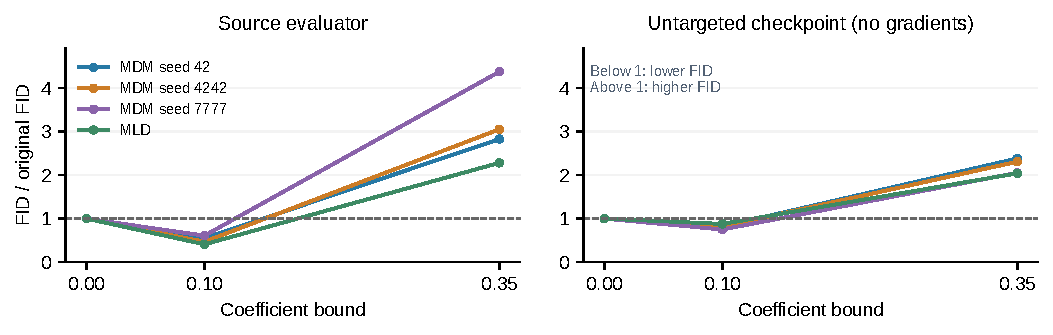
\includegraphics[width=\textwidth]{figures/blind_checkpoint_transfer.pdf}
\caption{\textbf{Caption-blind attacks transfer without destination gradients.} Every attacked output is sealed before reference scoring. Lines show FID divided by the same reader/cohort's original FID, for all tested bounds: source T2M weights on the left and another official checkpoint of the same architecture on the right. MLD supplies another generator; the three MDM cohorts overlap in source groups and are repetitions, not independent clip samples. Bound 0.1 helps every cohort; 0.35 harms every cohort.}\label{fig:blindtransfer}\end{figure*}

\begin{table*}[t]
\centering\footnotesize
\caption{\textbf{Sealed blind attacks on both generators and checkpoints.} FID for 960 outputs/cohort; both budgets, canonical-gradient and random controls. Destination checkpoint supplies no gradients. MDM groups overlap, so there is no pooled independent-clip interval.}\label{tab:blindtransfer}
\begin{tabular}{@{}llrrrrr@{}}\toprule
Cohort&Reader&Original&Bound0.1&Bound0.35&$C$ grad.&Random\\\midrule
mdm42&Source&0.3839&0.2099&1.0850&0.3839&0.3526\\
mdm42&Transfer&0.4083&0.3338&0.9718&0.4083&0.4965\\
mdm4242&Source&0.3762&0.1761&1.1477&0.3762&0.3231\\
mdm4242&Transfer&0.3710&0.3030&0.8555&0.3710&0.3790\\
mdm7777&Source&0.3268&0.1987&1.4292&0.3268&0.3011\\
mdm7777&Transfer&0.3793&0.2839&0.7786&0.3793&0.4319\\
mld&Source&0.7064&0.2886&1.6108&0.7064&0.6698\\
mld&Transfer&0.6594&0.5786&1.3452&0.6594&0.8104\\
\bottomrule\end{tabular}\end{table*}

MLD reuses the first 960 eligible outputs from native repetition 0 after excluding every original target-aware test source/mirror group. Selection is based on source identity, not scores. Segment names map to their underlying source before exclusion. The reference motion/captions are sealed separately; training targets, budgets 0.1/0.35 and 80-step final-iterate Adam match the MDM protocol. Native output durations, captions and reference crops remain paired. This is a new generator source but not a globally untouched test split.

The MLD source-reader FID changes 0.7064$\to$0.2886 at 0.1 and worsens to 1.6108 at 0.35. Canonical-gradient controls remain at baseline. Native reconstruction verifies 5,760 equivalent pairs and 48 FK samples; position/contact/velocity features stay bitwise unchanged. Maximum FK difference is $6.0\times 10^{-7}$ m.

All four sealed cohorts are then scored by the untargeted official T2M-GPT checkpoint, with the same architecture and normalization but distinct weights. No destination gradients, refitting or new target moments are used. At bound 0.1, MDM FID reductions are 18.2/18.3/25.1\%; MLD reduces 12.3\%. The larger budget worsens every cohort. Canonicalization closes the channel in the destination reader as well. These transfer changes are descriptive, not an independent-generator or population CI.

The two further MDM cohorts have 769 and 761 unique source groups; their intersection is 493. Their overlap with the first blind cohort is 494/496. Shared training targets and source overlap are disclosed; no pooled independent-clip interval is reported. FID changes are evaluator effects at identical represented movement, not improved generator quality.


\section{Canonical real-data sanity checks and portable implementation}
\begin{table}[t]
\centering\footnotesize
\caption{\textbf{Sanity check on already canonical real motion.} Twenty paired native draws. HumanML primary/secondary share an architecture; TMR differs. KIT uses its 251-feature evaluator. R1 equality is expected for already canonical rotations and does not establish accuracy cost on noncanonical inputs.}\label{tab:defensecost}
\begin{tabular}{@{}lrrr@{}}\toprule
Data/reader&Raw R1&$C$ R1&$C-$raw\\\midrule
HumanML primary&0.45275&0.45275&+0.00000\\
HumanML secondary&0.51222&0.51222&+0.00000\\
HumanML TMR&0.67842&0.67842&+0.00000\\
KIT primary&0.42443&0.42443&+0.00000\\
\bottomrule\end{tabular}\end{table}

Across 20 paired native draws, HumanML R1 raw/canonical is 0.45275/0.45275 for the primary T2M reader, 0.51222/0.51222 for the secondary reader and 0.67842/0.67842 for TMR. KIT real-motion R1 is 0.42443 in both paths. The paired R1 differences are exactly zero in these observations. Small floating-point embedding differences are measured separately. These real-motion rotations are already canonical. The unchanged retrieval therefore checks numerical implementation; it is not empirical evidence of a cost-free defense on noncanonical inputs. Matched sign-language reader adaptation is reported separately.

A portable NumPy implementation canonicalizes the two consecutive 3-vectors before evaluator normalization, validates the nondegenerate domain and preserves every nonrotation channel and padded frame bitwise. Tests cover arbitrary positive scale/shear, idempotence, orthogonality, both native schemas and invalid rotations. The accompanying evaluation contract specifies converter convention, input normalization, masking and reader-fitting/inference agreement. It closes only the 6D fiber; generic physical or cross-feature attacks remain possible.


\section{Sign-language data and readers}
Learned layers receive source text; final backtranslation consumes only features, lengths and masks. Raw/canonical evaluation of one output preserves rotations; comparisons between different generators do not.

\paragraph{Release and sample counts.}
We use the native SignSparK/SignSparK-BT converter, code, author BT checkpoints and released re-optimized motion. Pinned revisions and input fingerprints accompany the artifacts. Motion contains 240 raw 6D features per frame: body 60, left hand 90 and right hand 90. Left-hand features 60--149 are protected during attacks. The physical converter uses normalized orthogonal rows, not SVD projection.

Native valid train/dev/test counts are 7,096/519/642 PHOENIX, 29,630/1,650/2,183 How2Sign, and 18,201/1,064/1,162 CSL. Counts reflect the released loader, its 300-frame cap and filtering, not universal dataset sizes. Native text vocabularies, tokenization, normalization, beam search and punctuation are retained. CSL reader conditioning uses native segmented tokens; reported BLEU uses characters after removing spaces, preserving punctuation. Recognition supervision is disabled in BT fine-tunes; missing How2Sign pseudo-gloss files are therefore not inputs.

\paragraph{External evaluator scope.}
All public BTs share one Sign Language Transformer architecture. Whole-split real test raw scores are 14.9995, 3.4779 and 6.8907, versus release-card 15.00/3.53/6.98. Only PHOENIX matches after rounding. Replaying native/prepared features yields the same hypotheses; the cause of the other small differences is unresolved and decoding was not retuned to chase card scores.

\paragraph{Fitting and validation scope.}
Clip IDs are disjoint between fitting-split training and evaluated dev/test. Last-epoch selection applies to all fitted layers and readers. All development weights, outcomes and configurations are frozen before the fixed confirmation's inference, with no new fitting or test-based checkpoint selection. These public test splits had already been evaluated during the project; we do not claim project-wide untouched holdouts.


\section{Conditional output layers and budgets}
\begin{table*}[t]
\centering
\caption{\textbf{A learned layer increases scores without changing rotations.} PHOENIX TEST, 642 clips, three layer-training seeds. All generator/reader weights and layer checkpoints were fixed before confirmation; inference has no optimization. Canonical hypotheses remain identical in every condition. Gain intervals pair clips and condition on the three seeds.}
\label{tab:learned}
\begin{tabular}{lrrrr}\toprule
Output-layer training&Raw BLEU&Canonical BLEU&Raw gain&95\% gain interval\\\midrule
No layer&6.39&6.39&---&---\\
Text + motion / raw loss&15.21&6.39&8.81&$[7.82,9.87]$\\
Motion only / raw loss&7.60&6.39&1.21&$[0.66,1.76]$\\
Text + motion / canonical loss&6.26&6.39&-0.13&$[-0.32,0.04]$\\
\bottomrule\end{tabular}\end{table*}

\paragraph{Generated PHOENIX motion.}
A frozen geometry generator produces 7,096 train and 519 dev motions using text, capped reference duration, DDIM 50~\cite{song2021}, CFG 3~\cite{ho2022}, seed 102 and inference batch 16. No reference poses, glosses or anchors enter the sampler. Canonical outputs are cached; fixed test reuses 642 saved outputs of the same generator.

The 299,384-parameter layer copies the generator's frozen 128-wide text encoder, including eval-mode dropout. Motion projection 240 to 128, frame embeddings 300, four-head cross-attention, and three residual temporal convolutions (dilations 1/2/4, kernel 3, GroupNorm 8) feed a zero-initialized 120-channel head. Padding is masked after blocks; text cap 64. Bounded coefficients $q=B\tanh h$ produce $(e^{q_1}a,e^{q_2}b+q_3 a)$. Joints 10--24 are identity. Nine original fits cross three seeds with text/raw loss, motion/raw loss and text/canonical loss; all use 20 epochs, batch 64, AdamW 0.001, weight decay 0.0001, clipping 1 and matched minibatches. Final checkpoints are used. Source text is available to this amortized attack~\cite{gap2018,atn2018}; final reader decoding receives no text prefix.

Canonical-loss numerical drift is retained: raw gain 0.0058 dev/$-0.1347$ test, intervals containing zero. A circular text shift changes only layer conditioning; all 519 dev/642 test shifted captions differ. It raises agreement with that caption while lowering actual-caption BLEU, keeping canonical predictions identical. Exact train-caption overlaps are 25 dev/32 test; excluding them preserves positive gain, but does not test unseen vocabulary or signers.

\paragraph{Real How2Sign/CSL motion.}
Each corpus uses raw native real training features. The temporal stack is unchanged; source text uses native 512-wide reader embeddings (frozen), a fitted 512 to 128 projection and two 128-wide Transformer layers with dropout 0. Trainable parameters are 769,784. This is not the PHOENIX generator encoder or a language-transfer experiment. Caption tokens come from the native training input, capped at 64. Three seeds fit text/raw CE; one seed 42 fits each exploratory motion/raw and text/canonical control. The schedule matches the generated-motion layer.

\begin{table*}[t]
\centering\small
\caption{Native real-motion TEST layers and every control. Controls use one seed, so their intervals do not estimate seed variation. All canonical predictions stay fixed.}
\label{tab:realcontrols}
\begin{tabular}{llrrrrr}\toprule
Corpus&Objective&Seeds&Raw&Gain&Paired95\%&Seed+group95\%\\\midrule
How2Sign&Text / raw CE&3&6.11&2.64&$[2.27,3.03]$&$[2.24,3.06]$\\
How2Sign&Motion / raw CE&1&3.33&-0.14&$[-0.35,0.06]$&$[-0.35,0.06]$\\
How2Sign&Text / canonical CE&1&3.48&0.00&$[-0.18,0.20]$&$[-0.18,0.20]$\\
CSL-Daily&Text / raw CE&3&7.43&0.54&$[0.14,0.97]$&$[0.11,1.00]$\\
CSL-Daily&Motion / raw CE&1&6.74&-0.16&$[-0.64,0.29]$&$[-0.64,0.29]$\\
CSL-Daily&Text / canonical CE&1&6.79&-0.10&$[-0.40,0.09]$&$[-0.40,0.09]$\\
\bottomrule\end{tabular}\end{table*}

Full test primary gains are 2.6363 How2Sign, VIDEO\_ID interval $[2.2654,3.0291]$, and 0.5426 CSL, clip interval $[0.1436,0.9719]$. Seed-plus-group intervals remain positive. All canonical hypotheses are unchanged across primary/control models. Controls have one seed and cannot estimate training-seed variability. Raw-source motion is retained, rather than canonicalized before fitting; baseline canonical scores consequently differ from raw scores.

\paragraph{Small bounds and detectability.}
Nine additional PHOENIX fits use bounds 0.01/0.05/0.1 with the original three seeds and identical epochs/batches. Natural RMS is computed on the same generator's raw features; attack input is its canonical encoding. For each clip, RMS is $\sqrt{\operatorname{mean}(x-C (x))^2}$. The detector is a single threshold on this statistic. AUC reports the better of the two orientations, not a separate trained detector or a general privacy guarantee.

\begin{table*}[t]
\centering\small
\caption{Small-bound PHOENIX test layers, all three seeds; baseline 6.3905. RMS is distance to canonical features. Detector AUC uses the better threshold orientation against the same raw generator. At 0.05 the seed-sensitive gain interval includes zero.}
\label{tab:smallbudget}
\begin{tabular}{rrrrrrr}\toprule
Bound&Raw&Gain&Paired95\%&Seed+clip95\%&RMS&AUC range\\\midrule
0.01&6.44&0.05&$[-0.20,0.29]$&$[-0.22,0.32]$&0.0056&1.000--1.000\\
0.05&7.24&0.85&$[0.48,1.23]$&$[-0.01,1.68]$&0.0274&1.000--1.000\\
0.1&8.04&1.65&$[1.15,2.16]$&$[0.32,2.81]$&0.0548&0.917--0.941\\
\bottomrule\end{tabular}\end{table*}

Bound 0.05 has paired test gain interval $[0.4807,1.2343]$, but seed-plus-clip interval $[-0.0055,1.6770]$ includes zero. Bound 0.1 remains positive under seed sensitivity $[0.3189,2.8077]$. Test RMS-detector AUC is 1.00 at 0.01/0.05 and 0.917--0.941 at 0.1. The raw generator RMS is around 0.10; attacked RMS 0.027/0.055 can lie below it and still be separable. Lower norm distortion is not stealth.

\paragraph{Per-clip target-aware budgets.}
Sixty dev conditions cross four bounds, four iteration counts and three parameter granularities, with the available combinations retained exactly. Global coefficients, per-frame coefficients and per-frame/joint coefficients have sharply different capacity. Random transforms do not use targets. At 0.35/80 steps wrong-target BLEU is 0.9166/9.5845/83.3517 for global/frame/frame-joint; at 0.1 frame-joint gives 32.47. These searches use caption access at optimization time and are not production performance.

\begin{figure*}[t]
\centering
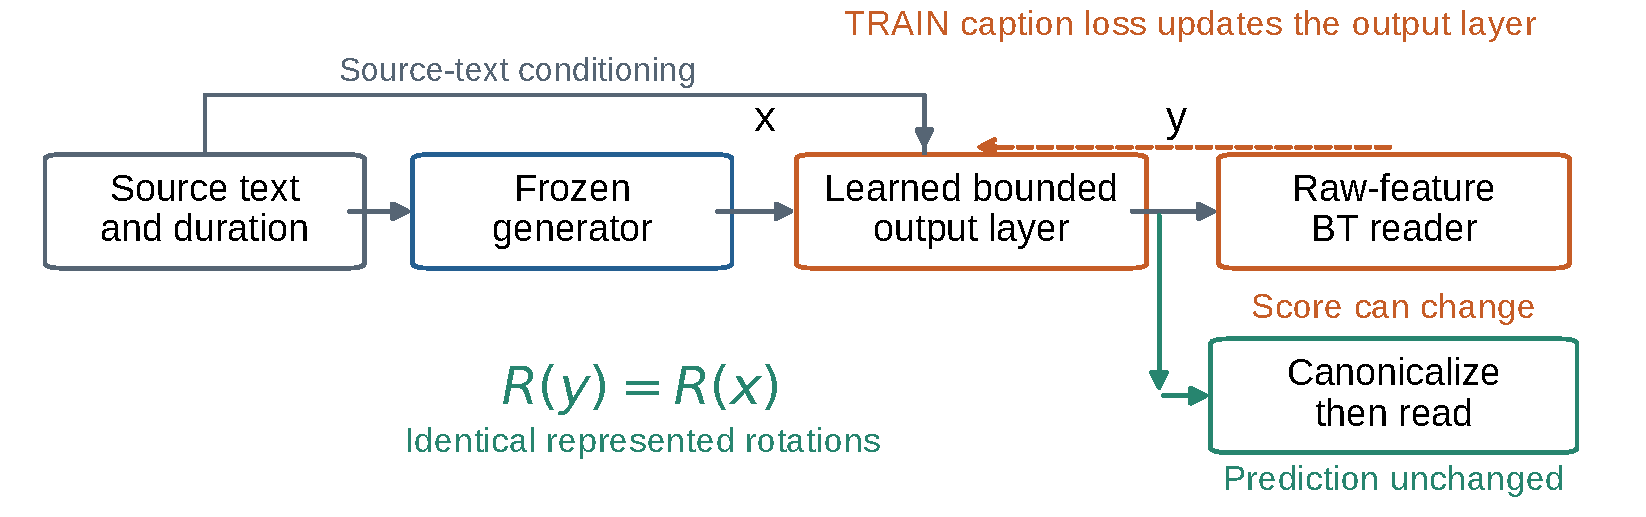
\includegraphics[width=\textwidth]{figures/learned_method.pdf}
\caption{\textbf{Learning changes the evaluation while the rotations stay fixed.} Source text and frozen generated motion condition a bounded output layer. Training-caption loss updates only that layer. At evaluation it performs one pass, with no per-clip search. The raw reader can respond to its coefficients; canonicalization removes them before reading. The three layer objectives use matched batches and initialization.}
\label{fig:learnedmethod}
\end{figure*}

\begin{figure}[t]\centering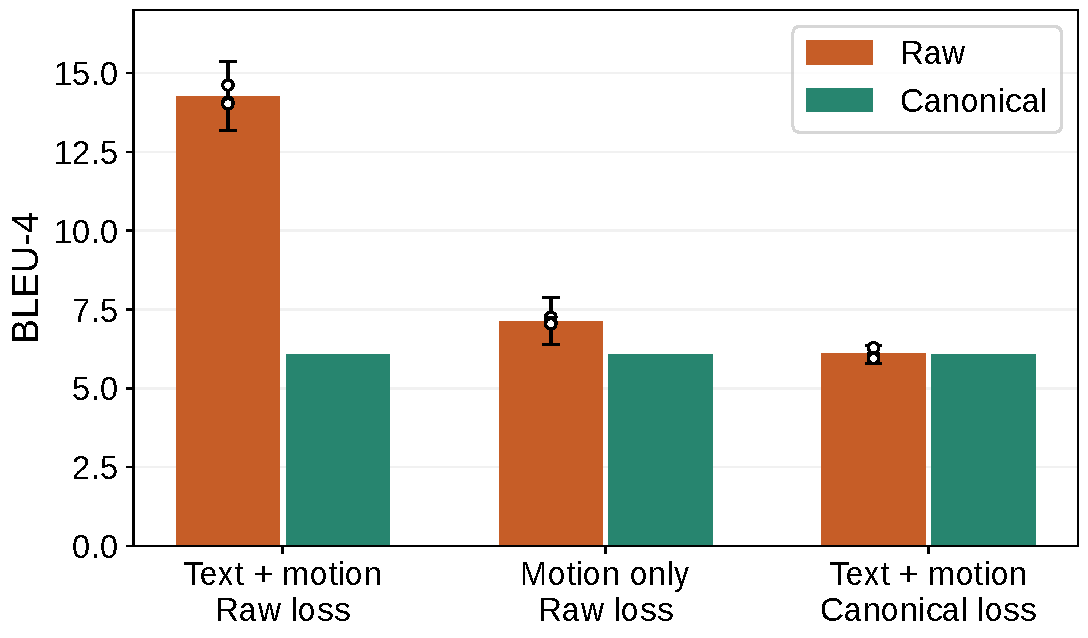
\includegraphics[width=\linewidth]{figures/learned_results.pdf}
\caption{\textbf{A learned channel on dev.} Bars average three seeds; dots show seeds. Whiskers are paired 95\% raw-gain intervals anchored at the fixed baseline. Canonical hypotheses are identical. Test results are in the main paper.}\label{fig:learnedresults}\end{figure}

\begin{figure*}[t]\centering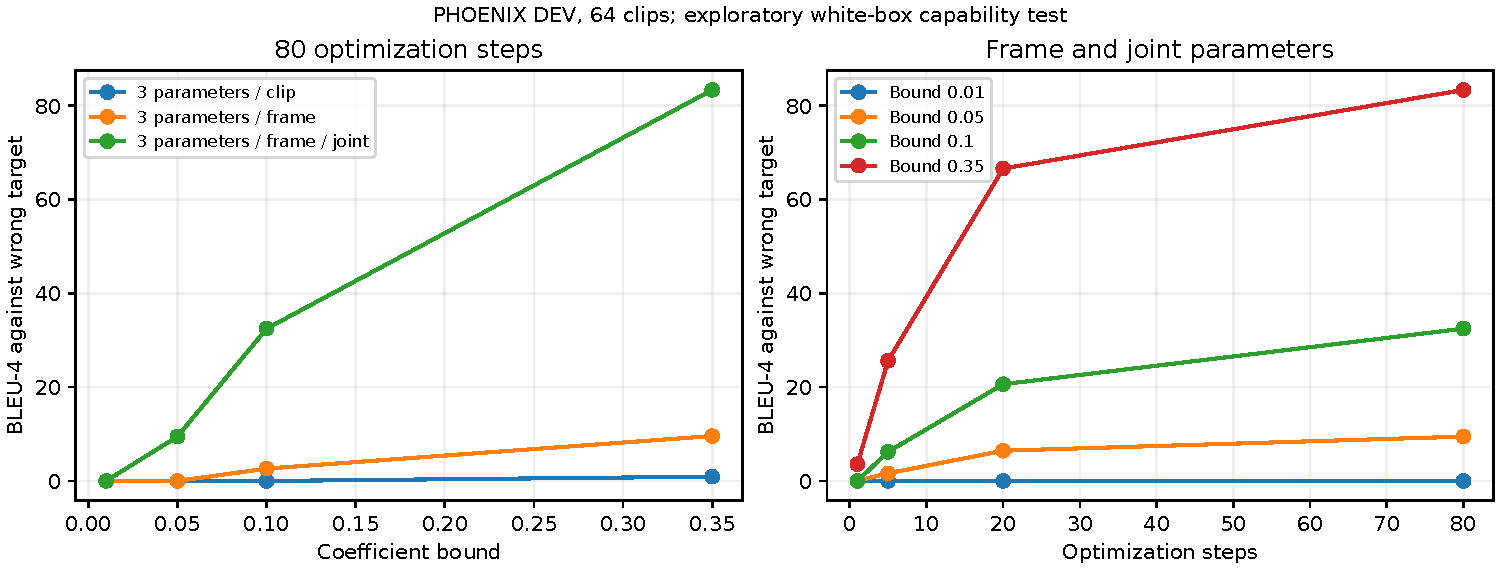
\includegraphics[width=\textwidth]{figures/attack_budget.pdf}
\caption{\textbf{Per-clip optimization budget on 64 PHOENIX dev clips.} Wrong-target BLEU depends on bound, steps and parameter granularity. Random controls are target-independent. These target-aware searches differ from learned-layer inference; all 60 conditions are retained.}\label{fig:attackbudget}\end{figure*}

\paragraph{Fixed recodings of generated sign motion.}
Four frozen local diffusion variants also generate 642 test motions each. Raw, canonical, fixed scales 0.9/1.1 and shear 0.1 are equivalent encodings with protected left hands, independent of captions. In the generated-near variant, scale 0.9 minus raw is $-0.6592$, family interval $[-1.2267,-0.0949]$; scale 1.1 minus 0.9 is +0.8554, family interval $[0.1734,1.5347]$. These 20-contrast, 20,000-resample results establish within-system representation effects. Between-generator opposite rank orderings are not supported as a primary claim. Geometry/velocity/reader-CE/generated-near variant definitions and raw arrays remain in the machine-readable evidence map.


\begin{table*}[t]\centering\small
\caption{Exact checkpoint SHA256 identifiers. The full hashes, configurations, dataset revisions and code snapshots accompany the artifacts.}\label{tab:hashes}
\begin{tabular}{ll}\toprule
Checkpoint & SHA256\\\midrule
PHOENIX BT & \texttt{80c67168ddadcc6f0517ea995dd9340da6c4f3e424bb667197d9282ce4774279}\\
How2Sign BT & \texttt{acf8794c594f9b58701c85c390264cf30807d89f399960768f30c7a9e637e01f}\\
CSL BT & \texttt{5ea787537b11d7b3e14e6a5c3ae711931b8abf939f6a7f25e5a9b8dd3e91a2c0}\\
Local CTC & \texttt{32e5c1022e5b753c0b7943df0ce52c177eef8e82cebc92cea3a620eec21f7556}\\
Geometry & \texttt{c78566bace1113358eacde2aeed47cc4f157bb83eb3d8bfb22b1d325d9b9f66d}\\
Velocity & \texttt{ec72aa705bec2fd46b2f41718b0a349e43385a7b270d056bf766d0c71ae9e8f2}\\
Reader CE & \texttt{ed5799d024dd4bde095d04908fe39a85b69117ce49f697f268ddb19a659b79ae}\\
Generated near & \texttt{ae7bd92c0f99ebb55d54591e89543d8d0a68ec995821c255402c48377b3fe52f}\\
Shared initial DDPM & \texttt{abdddac25d5e63887242e9af08ac440c2929617f26cff947b5a2a023f3bc8ae1}\\
\bottomrule\end{tabular}\end{table*}



\section{Adaptive per-clip detector-statistic tests}
\paragraph{Fixed-distance and fixed-norm surfaces.}
For fixed rows $u,v$, write $s=(\rho-1,\sigma-1,\tau)$. Squared distance to canonical features is
\begin{equation}
E=\|d-C (d)\|^2=\|s\|^2.
\end{equation}
Any auxiliary rotation $Q$ of $s$ preserves $E$. If $\|s\|<0.95$, reconstructed $\rho',\sigma'>0.05$; otherwise the layer returns the identity. This auxiliary rotation changes redundant scalars, not physical joint rotations.

Squared 6D norm $N=\rho^2+\sigma^2+\tau^2$ obeys
\begin{equation}
N-E=2 (\rho+\sigma)-2.
\end{equation}
A rotation around $(1,1,0)/\sqrt 2$ additionally preserves $\rho+\sigma$, hence both $N$ and $E$ per frame/joint: the representatives with fixed $E$ and $N$ form a circle. Rotations about arbitrary axes preserve $E$ only and form a sphere. Positive-scale safety, padding and left-hand protection apply to both.

The auxiliary-coordinate geometry is distinct from physical joint rotation or an intrinsic diffusion process.

\begin{figure*}[t]\centering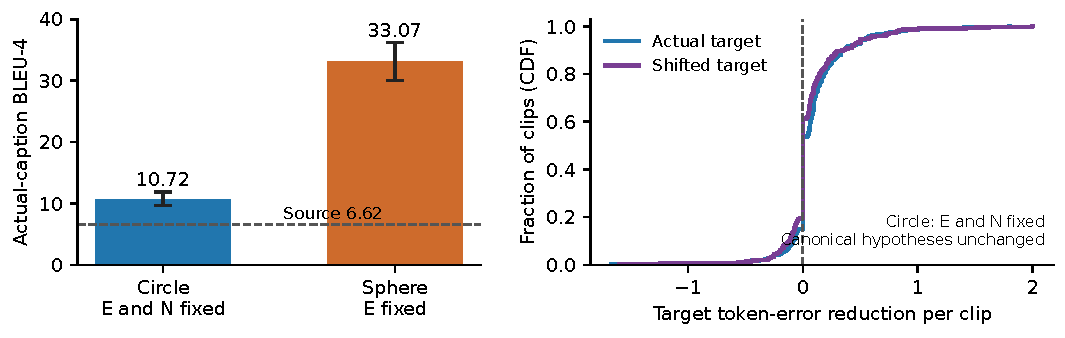
\includegraphics[width=\textwidth]{figures/adaptive_statistics.pdf}
\caption{\textbf{Adaptive attack at fixed detector statistics.} Left: PHOENIX actual-caption BLEU and family-adjusted gain intervals. Right: per-clip reduction in target-normalized token edit error. The circle preserves canonical distance and squared feature norm per joint/frame while canonical hypotheses remain fixed. The sphere preserves distance alone. These are target-aware capability tests, not general stealth.}\label{fig:supadaptivestatistics}\end{figure*}
Dev 64 is selected uniformly with seed 20261012 before the new per-clip optimization; it uses the frozen generator's raw dev outputs. Both 80- and 200-step endpoints are retained. Full test 642 confirmation fixes the final 200-step endpoint and four geometry/target conditions before inference. Source motions come from the existing raw generator archive; no real reference pose is used to generate them. Raw source BLEU is 6.62 here, versus 6.39 for the canonical input of the learned-layer study, for the same represented motion.

Optimization uses Adam 0.1, zero-initialized per-frame/joint coefficients and frozen BT weights. A scalar $q$ predicts circle phase $\pi\tanh q$, bounded by $\pi$. Sphere coordinates are $(\pi/\sqrt 3)\tanh q_i$, giving auxiliary rotation magnitude at most $\pi$. Radius $\ge 0.95$ remains identity, and left-hand joints 10--24 remain byte-identical. Target captions are either the original source or the fixed circular shift; all 642 test shifts differ. No decoded-score checkpoint selection occurs.

\begin{table*}[t]\centering\small
\caption{\textbf{Adaptive per-clip attacks, full PHOENIX TEST642.} All four final 200-step endpoints. Circle preserves canonical distance $E$ and 6D norm $N$ per joint/frame; sphere preserves only $E$. Intervals adjust for four target-gain comparisons. Target text is explicitly provided; these are neither learned-layer transfer nor ordinary training.}
\label{tab:adaptivestats}
\begin{tabular}{llrrrr}\toprule
Surface & Target caption & Before & After & Gain & Family 95\% CI\\\midrule
Circle & Actual & 6.62 & 10.72 & 4.09 & [3.04, 5.24]\\
Circle & Shifted & 1.25 & 3.35 & 2.10 & [1.22, 3.12]\\
Sphere & Actual & 6.62 & 33.07 & 26.45 & [23.46, 29.52]\\
Sphere & Shifted & 1.25 & 22.51 & 21.27 & [18.50, 24.22]\\
\bottomrule\end{tabular}\end{table*}


On dev 64, circle actual-caption BLEU is 6.59 to 10.06 at 200 steps, gain 3.46; its eight-endpoint-adjusted interval is $[1.15,6.49]$. Circle wrong-target gain is 2.82, with lower adjusted endpoint zero. Sphere actual/wrong-target gains are 26.79/20.72, with adjusted intervals $[17.09,37.53]$/$[11.93,31.93]$. These dev results motivated prospective fixed test confirmation; they are not pristine validation.

Test circle gains are 4.09 actual and 2.10 shifted, with four-comparison-adjusted intervals $[3.04,5.24]$/$[1.22,3.12]$. Sphere gains are 26.45/21.27, intervals $[23.46,29.52]$/$[18.50,24.22]$. Random coefficient controls use fixed seeds 42/123/777 per surface. Canonical-reader CE optimization is run for 200 steps per surface. Their wrong-target gain intervals do not exclude zero on the positive side. Every source/target, full loss trace and output array is retained; randomization seeds are not independent training seeds.

RMS threshold AUC is 0.5003 for the circle and 0.5007 for the sphere. The circle preserves both statistics; the sphere does not preserve feature norm and may be detectable by it. Preservation of $E,N$ is not indistinguishability of all redundant-coordinate distributions. Geometric invariants, decoded canonical strings, finite values and reconstruction are verified independently. Complete numerical residuals and source hashes accompany the results.

\paragraph{Other fixed-rotation attack capabilities.}
\begin{table}[t]
\centering\small
\caption{\textbf{Wrong-caption attacks at fixed rotations.} Each row uses 128 real test clips and target-aware optimization. Columns report BLEU-4 against the shifted target or actual caption. Scores across languages use distinct tokenization.}
\label{tab:wrongtargets}
\begin{tabular}{lrrrr}\toprule
&\multicolumn{2}{c}{Wrong target}&\multicolumn{2}{c}{Actual caption}\\
Corpus&Before&After&Raw after&Canon. after\\\midrule
PHOENIX&0.00&85.19&0.00&13.95\\
How2Sign&1.23&47.34&0.00&4.76\\
CSL-Daily&0.67&32.44&1.26&8.10\\
\bottomrule\end{tabular}\end{table}

Wrong-caption optimization reaches 85.19 PHOENIX BLEU against an incorrect target and zero against the actual caption (\cref{tab:wrongtargets}). How2Sign/CSL show the same failure with different token conventions. Three CSL targets duplicate actual captions and remain included. These are attack capability scores, not production quality.

The CTC model's wrong-target WER falls from 118.07\% to 3.76\%, while actual-reference WER reaches 121.58\%. Reversal or identity hands raises full test WER from 50.11\% to 91.48\% or 93.95\%. It responds to physical changes and redundant coordinates. All 1,024 BT/CTC attack pairs preserve canonical hypotheses.




\paragraph{Additional scalar detectors and the limit of statistic matching.}
An exploratory diagnostic fits scalar thresholds on dev 64 source/attacked clips and applies their fixed orientation/threshold to test 642. All nine statistics are reported: canonical RMS, mean squared 6D norm, means of $|\tau|$, $|\rho-\sigma|$, $\rho$, $\sigma$, and standard deviations of $\rho,\sigma,\tau$. Circle test AUCs span 0.500--0.530 with dev-fitted orientation; test balanced accuracies span 0.500--0.521. Sphere statistics are more informative: $|\rho-\sigma|$ AUC is 0.877 and balanced accuracy 0.801, with source false-positive rate 0.319 and attack detection rate 0.922. These post-hoc diagnostics are not independently validated security guarantees, and do not cover temporal, joint-wise or learned multivariate detectors.

For fixed canonical rows, the full Gram matrix of $(a,b)$ is
\begin{equation}
\begin{pmatrix}\rho^2&\rho\tau\\\rho\tau&\sigma^2+\tau^2\end{pmatrix}.
\end{equation}
Fixing all three entries determines positive $\rho,\sigma$ and $\tau$, hence the original features. Thus preserving $E,N$ leaves a circle, whereas fixing the entire Gram matrix at unchanged rotation leaves no channel. This elementary limit prevents interpreting two-statistic matching as general invisibility. It does not prove a practical detector's performance without evaluating that detector.

\begin{figure*}[t]\centering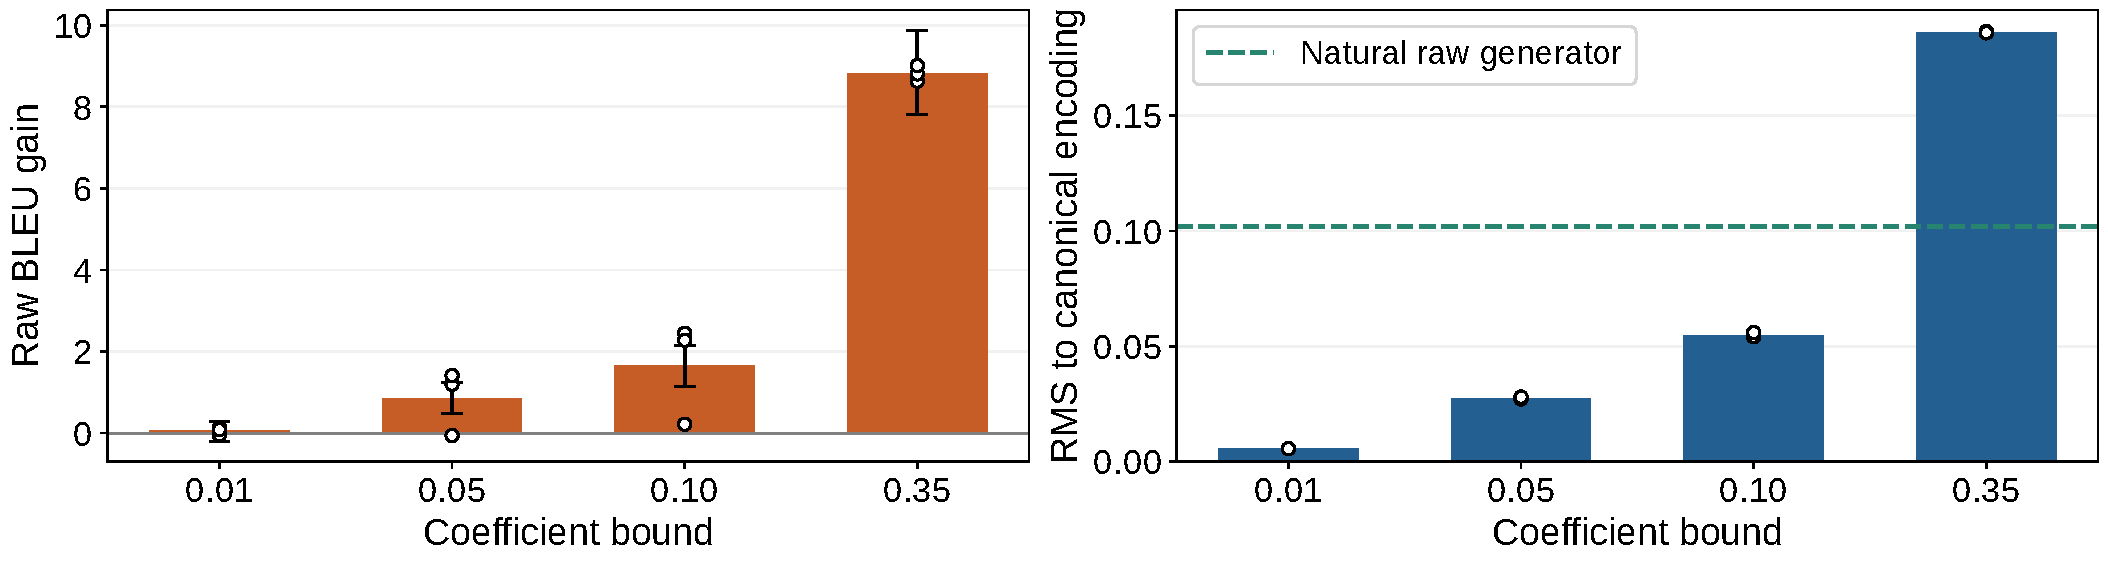
\includegraphics[width=\textwidth]{figures/learned_budget.pdf}
\caption{\textbf{Learned-layer budget on full PHOENIX test.} Left: mean raw gains, paired 95\% intervals and individual seeds. Right: RMS distance to canonical features, against the same raw generator's natural output. A scalar RMS detector separates most attacked outputs. Rotations/canonical hypotheses stay fixed; smaller magnitude is not undetectability.}\label{fig:learnedbudget}\end{figure*}


\section{Canonicalizing real sign inputs}
\begin{table*}[t]
\centering\small
\caption{\textbf{Natural dependence in real sign inputs, no attack.} Full native test with common loader preprocessing and frozen raw reader; no source-conditioned layer, optimization or new decoding. The shared left-hand preprocessing precedes both paths. Hypothesis counts and six BLEUs are independently recomputed; the CSL score is character-level.}\label{tab:signnatural}
\begin{tabular}{@{}llrrrr@{}}\toprule
Corpus&Changed / clips&Changed \%&Raw BLEU&$\C$ BLEU&$\C-$raw\\\midrule
PHOENIX&0/642&0.0\%&14.9995&14.9995&+0.0000\\
How2Sign&1,438/2,183&65.9\%&3.4779&3.4840&+0.0062\\
CSL-Daily&464/1,162&39.9\%&6.8907&7.0662&+0.1755\\
\bottomrule\end{tabular}\end{table*}

The same frozen raw reader decodes each real input and its canonical representative. There is no learned layer, source-caption conditioning, per-clip optimization or new model fitting. The results use the saved full native test hypotheses. Both paths share the original native preprocessing, including projection of left-hand channels 60:150 before decoding. Thus ``raw'' denotes the audit input under that shared preprocessing, not untouched bytes of the public release.

Independent code compares all 3,987 pairs of saved strings and recalculates the six corpus BLEUs from clipped n-gram counts and brevity penalties. PHOENIX changes 0/642 hypotheses; How2Sign changes 1,438/2,183; CSL changes 464/1,162. Scores use word tokens for PHOENIX/How2Sign and characters with punctuation retained for CSL. The full changed fractions are 0\%, 65.9\% and 39.9\%. Small corpus-score differences do not imply sentence-level invariance, improved semantics or an accuracy-free defense. Reader adaptation on noncanonical inputs is reported separately.


\section{Canonical-reader adaptation and independent recognizer}
\paragraph{Reader adaptation.}
Twelve fits cross How2Sign/CSL, three seeds and raw/canonical training input. Matched pairs share public initialization and batch/dropout choices. Five epochs, batch 64, AdamW $10^{-5}$, weight decay $10^{-4}$ and last-checkpoint selection apply. Both use translation CE, with recognition loss disabled. Canonical readers receive canonical features during training and decoding. Raw adaptation controls for the effect of fine-tuning itself.

Dev canonical-minus-raw differences are $-0.0620$ How2Sign/+0.1577 CSL; seed-plus-group intervals $[-0.2646,0.1424]$/$[-0.1529,0.5316]$. test differences are +0.0991/$-0.0217$, intervals $[-0.0332,0.2493]$/$[-0.2261,0.1859]$. Exploratory margins 0.2/0.3 BLEU are sensitivity choices, not human-equivalence thresholds. How2Sign does not establish noninferiority to its original public reader under seed-plus-group uncertainty; closure is not uniformly free accuracy.

Fresh 64-clip dev attacks per seed/arm/corpus use 80 Adam steps, learning rate 0.1 and bound 0.35. All 384 canonical-reader pairs preserve hypotheses; nonzero wrong-target BLEU can reflect shared n-grams in unchanged predictions. Independent reconstruction verifies 768 raw/canonical attack pairs. Fixed equivalent test encoding (scale 1.1, shear 0.1, protected left hand) preserves all 10,035 canonical-reader hypotheses.

\paragraph{Local CTC architecture and inference.}
The 2,562,867-parameter recognizer has a 1075-entry gloss vocabulary, two 128-channel temporal convolutions (kernel 5,stride 2), a two-layer bidirectional 256-unit GRU and greedy CTC head~\cite{graves2006}. Training normalization has std floor 0.05 and remasked padding. Training uses 7096 clips, batch 64, AdamW 0.001, cosine decay over 40 epochs, clipping 1 and seed 42; dev best WER is epoch 21. CuDNN is disabled consistently to support recurrent input gradients. Empty glosses retain insertion errors in micro-WER; one infeasible shifted CTC target is retained with zero-infinity loss, not removed.

\paragraph{Per-clip attack and feature-only decoding.}
BT minimizes target-token CE and CTC minimizes gloss CTC loss, with model weights frozen. Coefficients begin at zero and use bound 0.35. Selections are uniform without replacement, seed 2027, sorted by dataset index. CSL has three shifted-caption collisions retained. Final BT uses autoregressive decoding, not teacher forcing. A separate 768-hypothesis CSL replay forbids teacher-forced forward, asserts exactly features/lengths/masks at inference, and loads references only after predictions; every hypothesis matches the saved result. This is an input-contract check, not another independent performance experiment.


\section{Statistics, presentation and reproducibility}
Corpus BLEU is recomputed from clipped 1--4 gram counts, native tokenization and brevity penalty~\cite{papineni2002,post2018}. CSL removes spaces and preserves punctuation. A standard-library Counter implementation reproduces saved scores to $10^{-10}$. WER is verified by full-matrix edit distance and micro aggregation. Attack scores against wrong captions remain separate from actual-reference scores.

New intervals use 20000 paired bootstrap draws, seed 42, recomputing corpus metrics from sufficient statistics. How2Sign uses official VIDEO\_ID groups (115 dev/149 test), not verified signer identity. Within each sampled unit set, model-specific scores are computed separately before averaging differences across seeds. Sensitivity analysis resamples the three training seeds, all sharing one initialization; it does not estimate pretraining variation. One-seed controls have no seed uncertainty. Target-independent representation intervals cover 20 contrasts. Layer and budget intervals are nominal per contrast. Shifted-caption mappings remain fixed during resampling. Target-aware 128-clip audit intervals use 2000 draws and do not estimate training-seed variability.

The teaser uses the first fixed HumanML3D MDM record and procedural body geometry from native RIC positions. Original/recoded body pixels match exactly under the same camera and radii; rotations are verified numerically. Its retrieval values summarize 1,024 clips rather than the illustration.



\clearpage
{\small\bibliographystyle{ieeenat_fullname}\bibliography{references}}
\end{document}
